
\documentclass[11pt,compress,t,notes=noshow]{beamer}

\usepackage[english]{babel}
\usepackage{dsfont}
\newcommand\bmmax{2}
\usepackage{bm}
\usepackage{bbm}
\usepackage{verbatim}
\usepackage{amsmath}
\usepackage{amsfonts}
\usepackage{csquotes}
\usepackage{multirow}
\usepackage{longtable}
\usepackage{enumerate}
\usepackage[absolute,overlay]{textpos}
\usepackage{psfrag}
\usepackage{algorithm}
\usepackage{algorithmicx}
\usepackage{algpseudocode}
\usepackage{eqnarray}
\usepackage{multimedia}
\usepackage{media9}
\usepackage{arydshln}
\usepackage{tabularx}
\usepackage{placeins}
\usepackage{tikz}
\usepackage{setspace}
\usepackage{wrapfig}
\usepackage{tcolorbox}
\usepackage[export]{adjustbox}
\usepackage{siunitx}
\usetikzlibrary{shapes,arrows,automata,positioning,calc}
\tikzset{
  %Define standard arrow tip
  >=stealth',
  %Define style for boxes
  punkt/.style={
    rectangle,
    rounded corners,
    draw=black, very thick,
    text width=6.5em,
    minimum height=2em,
    text centered},
  % Define arrow style
  pil/.style={
    ->,
    thick,
    shorten <=2pt,
    shorten >=2pt,}
}
\usepackage{subfig}

%new environments

\newenvironment{vbframe}  %frame with breaks and verbatim
{
 \begin{frame}[containsverbatim,allowframebreaks]
}
{
\end{frame}
}

\newenvironment{vframe}  %frame with verbatim without breaks (to avoid numbering one slided frames)
{
 \begin{frame}[containsverbatim]
}
{
\end{frame}
}

\newenvironment{blocki}[1]   % itemize block
{
 \begin{block}{#1}\begin{itemize}
}
{
\end{itemize}\end{block}
}

\newenvironment{fragileframe}[2]{  %fragile frame with framebreaks
\begin{frame}[allowframebreaks, fragile, environment = fragileframe]
\frametitle{#1}
#2}
{\end{frame}}


\newcommand{\myframe}[2]{  %short for frame with framebreaks
\begin{frame}[allowframebreaks]
\frametitle{#1}
#2
\end{frame}}

\newcommand{\remark}[1]{
  \textbf{Remark:} #1
}

%%%%%%%%%%%%%%%%%%%%%%%%%%%%%%%%%%%%%%%%%%%%%%%%%%%%%%%%%%%%%%%%%%%%%%%%%%%%%%%

% basic latex stuff
\newcommand{\pkg}[1]{{\fontseries{b}\selectfont #1}} %fontstyle for R packages
\newcommand{\lz}{\vspace{0.5cm}} %vertical space
\newcommand{\dlz}{\vspace{1cm}} %double vertical space
\newcommand{\oneliner}[1] % Oneliner for important statements
{\begin{block}{}\begin{center}\begin{Large}#1\end{Large}\end{center}\end{block}}


%\usetheme{lmu-lecture}
\usepackage{../style/lmu-lecture}

\let\code=\texttt
\let\proglang=\textsf

\setkeys{Gin}{width=0.9\textwidth}


\title{Deep Learning}
\author{Mina Rezaei}
\institute{Department of Statistics -- LMU Munich}
\date{Winter Semester 2021}

\setbeamertemplate{frametitle}{\expandafter\uppercase\expandafter\insertframetitle}

%\begin{document}
%\sloppy
%\end{document}


\input{../../latex-math/basic-math}
\input{../../latex-math/basic-ml}
\input{../../latex-math/ml-nn}

\begin{document}

\lecturechapter{5}{Introduction CNNs}
\lecture{Deeplearning}
%%%%%%%%%%%%%%%%%%%%%%%%%%%%%%%%%%%%%%%%%%%%%%%%%%%%%%%

\begin{frame}
\frametitle{Lecture outline}
\tableofcontents
\end{frame}

\begin{vbframe}{Convolutional neural networks}
  \begin{itemize}
    \item Convolutional Neural Networks (CNN, or ConvNet) are a powerful family of neural networks that are inspired by biological process in which the connectivity pattern between neurons resembles the organization of the mamel visual cortex.
    \end{itemize}
 \begin{figure}
    \centering
    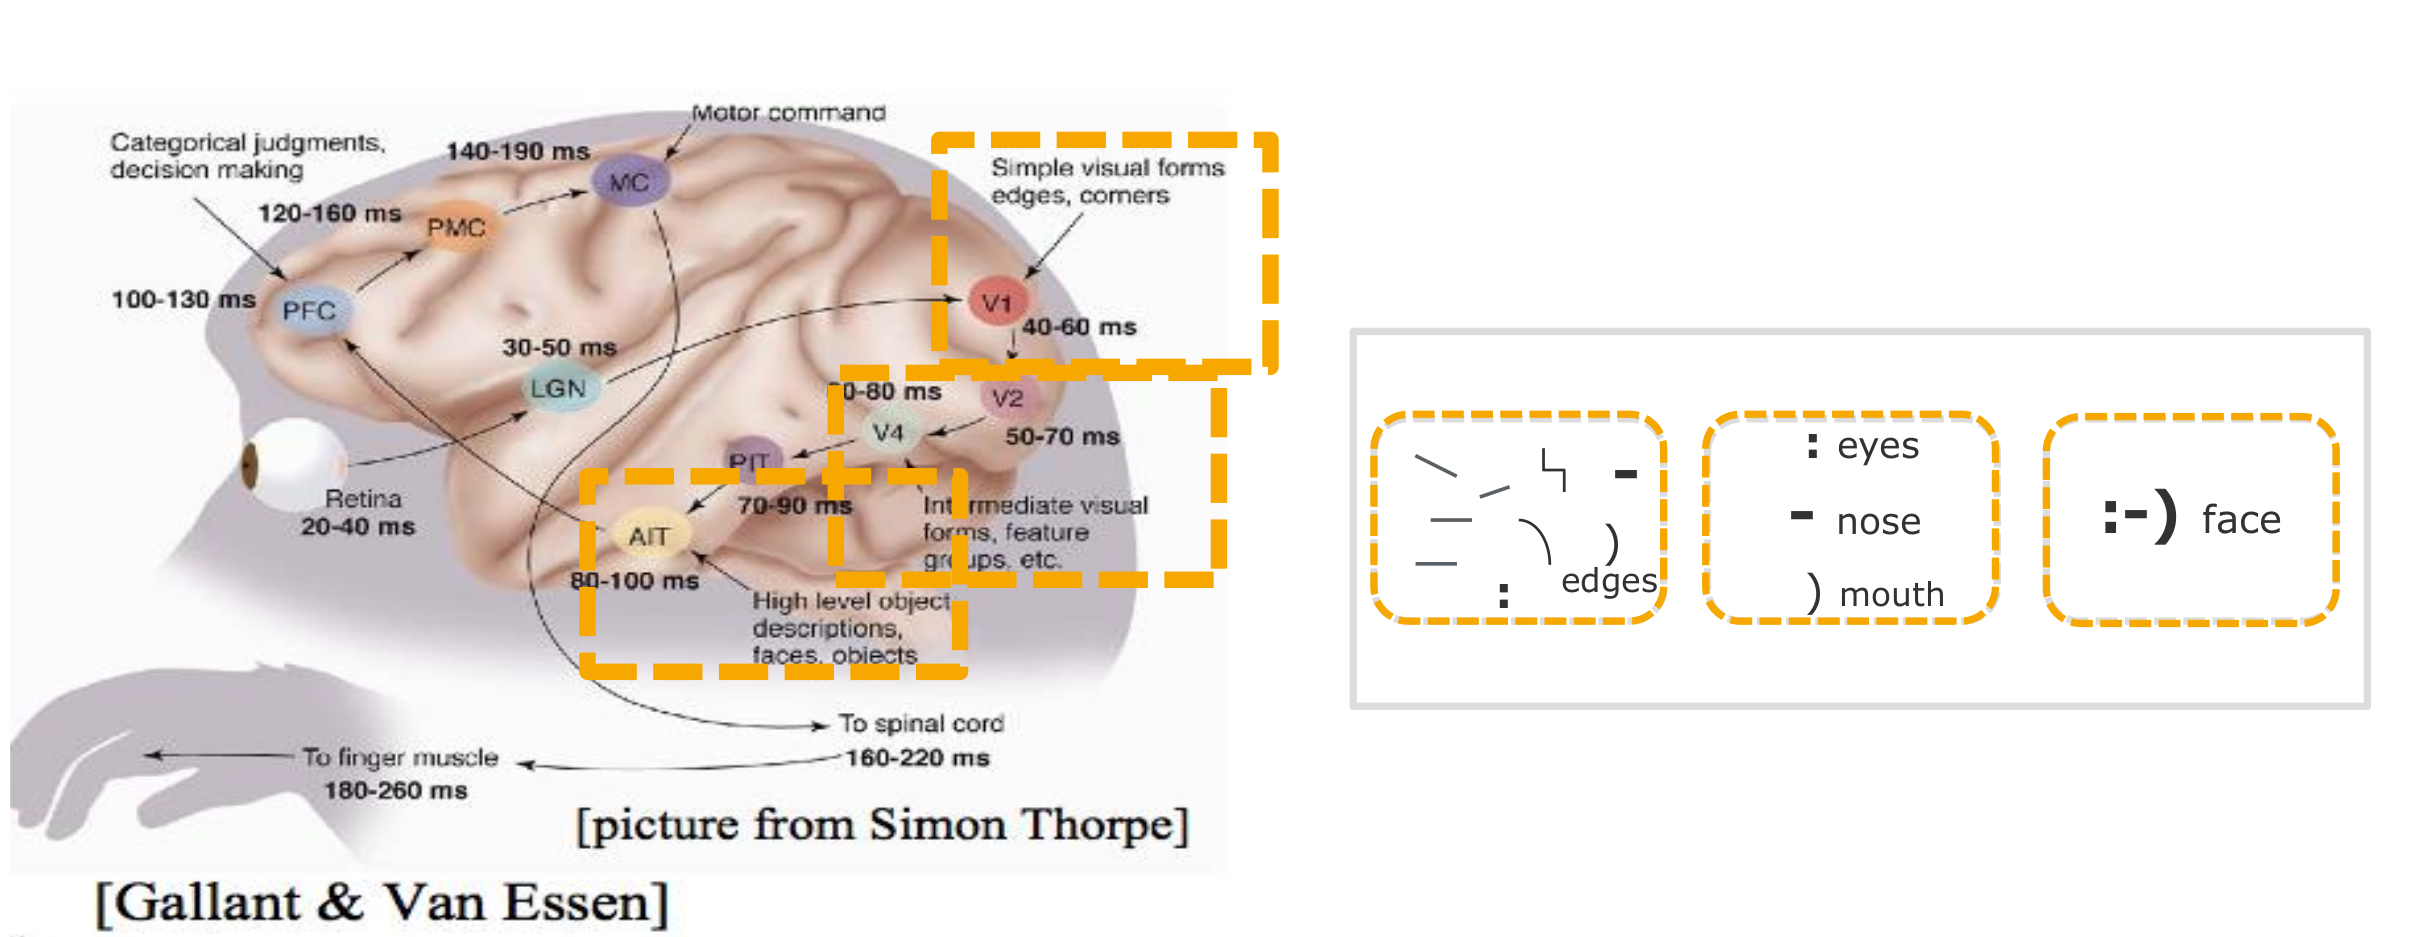
\includegraphics[width=8cm]{plots/cortex.png}
    \caption{The ventral (recognition) pathway in the visual cortex has multiple stage: Retina - LGN - V1 - V2 - V4 - PIT - AIT ...., lots of intermediate representations}
  \end{figure}
  
    \begin{itemize}
    \item Since 2012, by the success of CNNs model in ImageNet compition, they are state-of-the-art in many fields such as computer vision.
    \item Common applications of CNN-based architectures in computer vision are:
    \begin{itemize}
      \item Image classification.
      \item Object detection /localization.
      \item Semantic segmentation.
    \end{itemize}
    \item Also widely applied in other domains such as natural language processing (NLP), Speech and even time-series data.
    \item Basic idea: a CNN automatically extracts visual, or, more generally, spatial features from an input such that it is able to make the optimal prediction based on those features.
    \item Therefore, it contains different building blocks...
  \end{itemize}
\end{vbframe}


\section{CNN - Applications}

%%%%%%%%%%%%%%%%%%%%%%%%%%%%%%%%%%%%%%%%%%%%%%%%%%%%%%%%%%%%%%%%%%
%%%%%%%%%%%%%%%%%%%%%%%%%%%%%%%%%%%%%%%%%%%%%%%%%%%%%%%%%%%%%%%%%%
\begin{vbframe}{CNNs - What for?}
  \begin{figure}
    \centering
    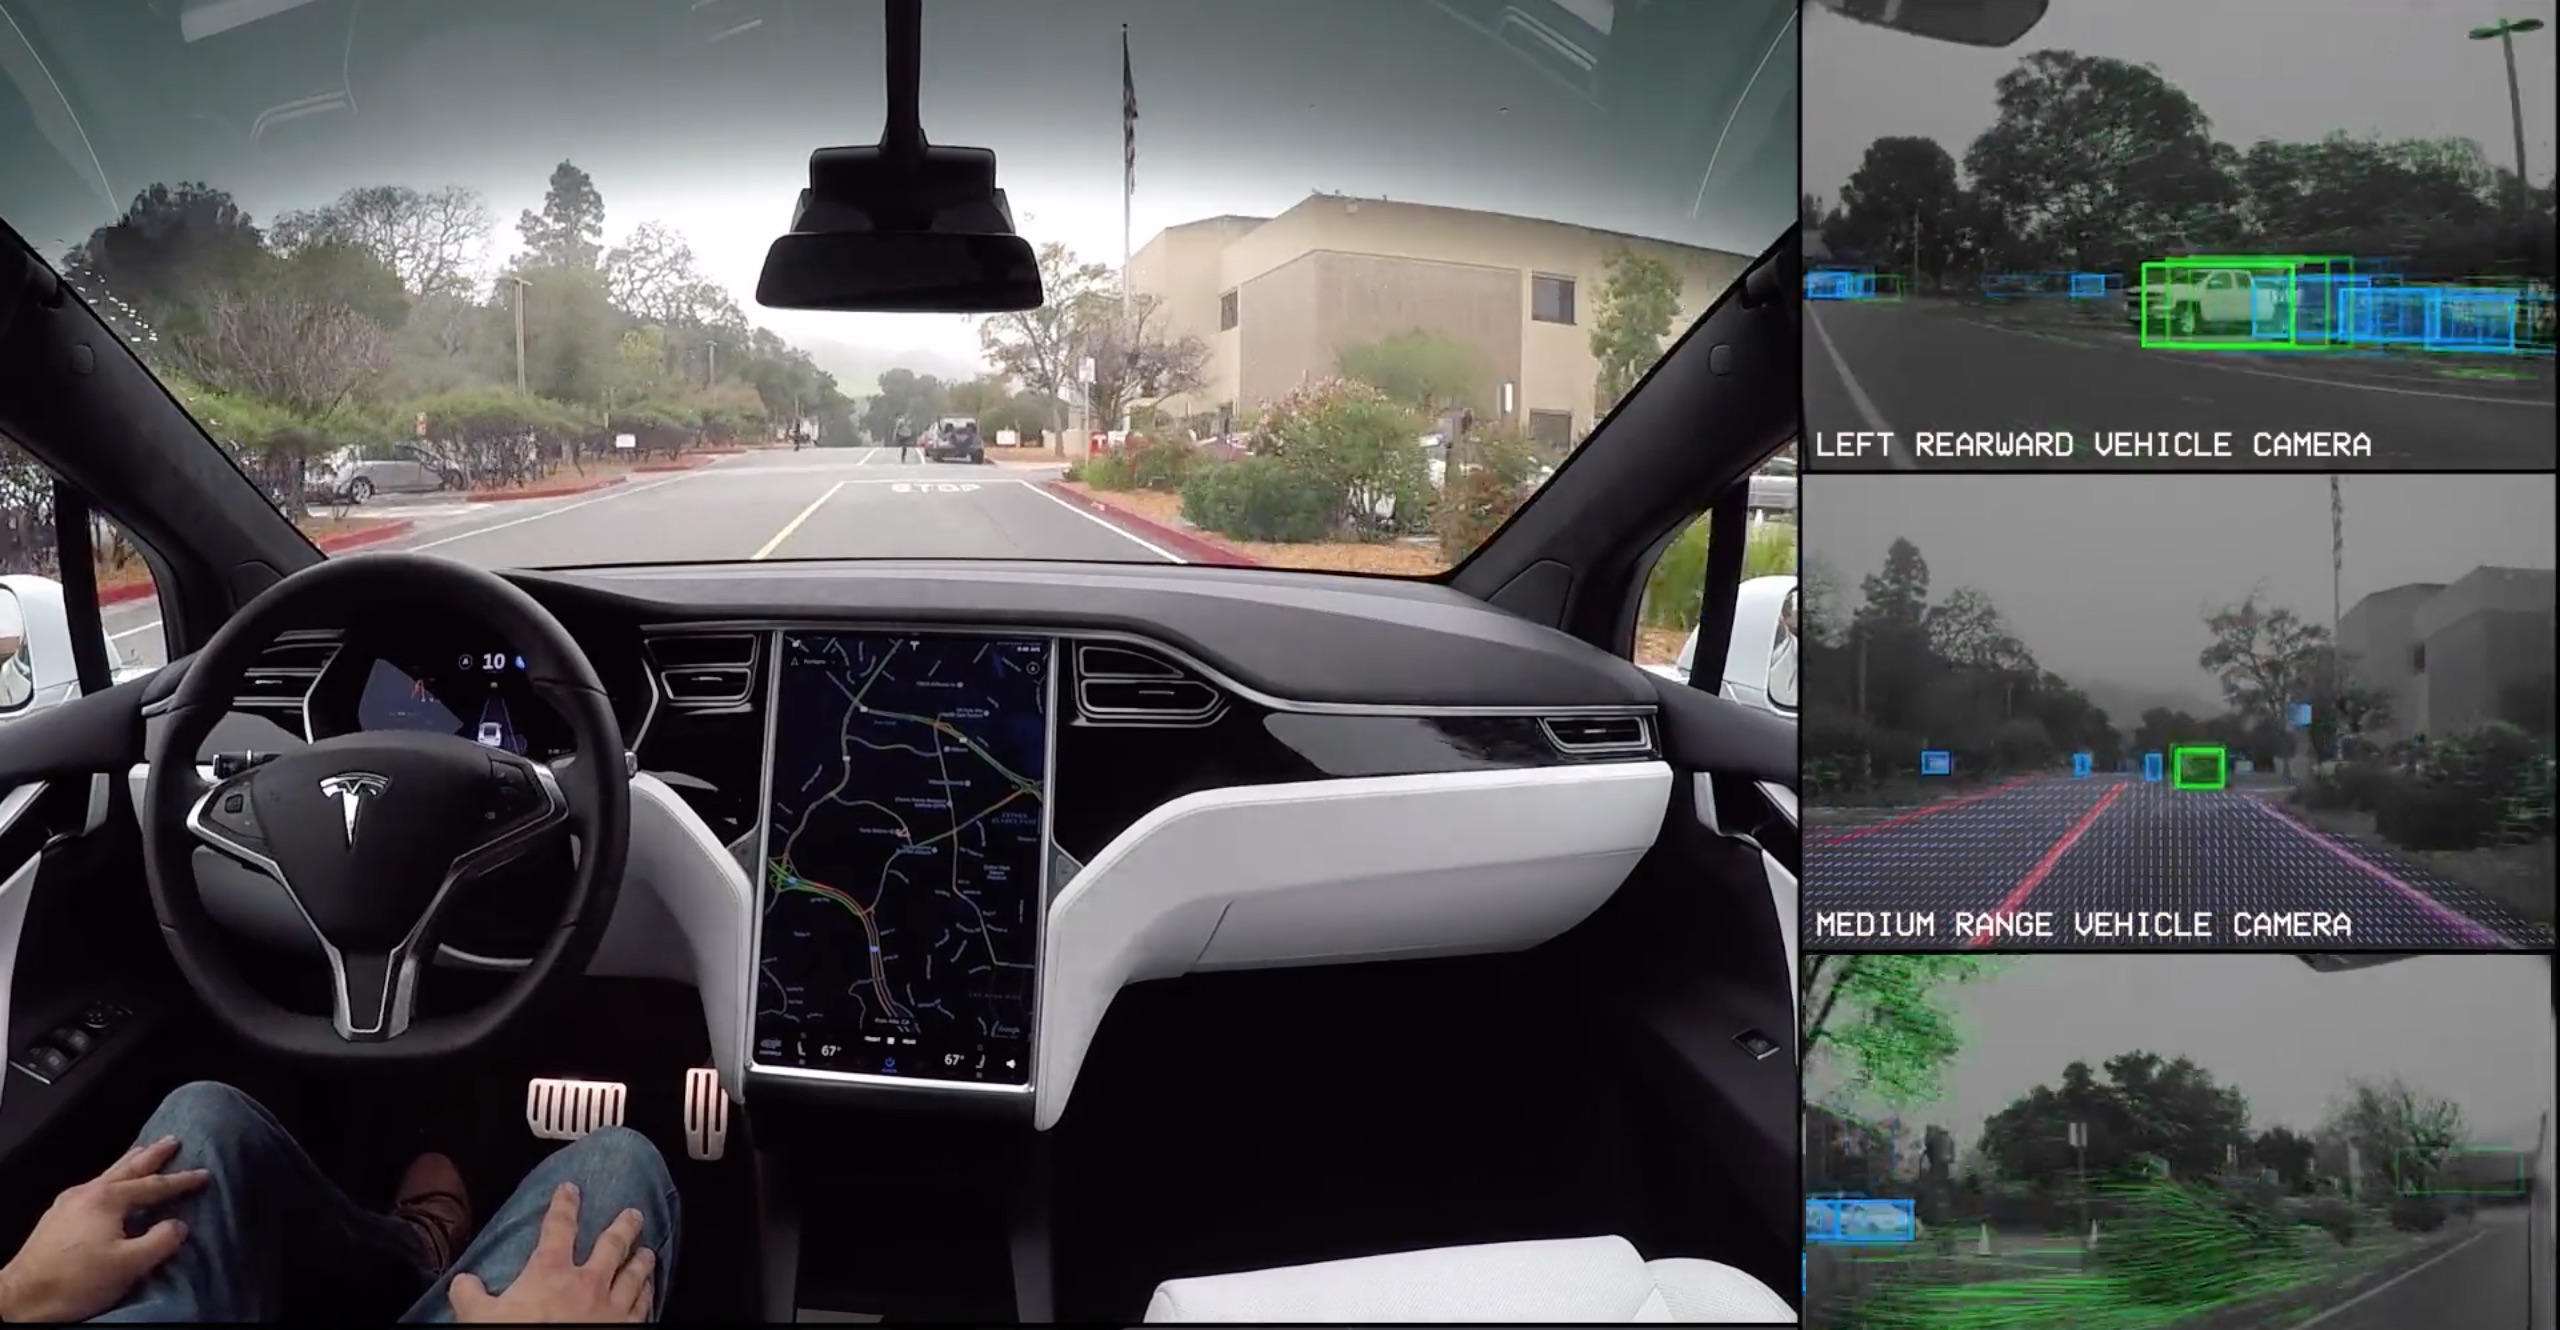
\includegraphics[width=7cm]{plots/tesla_autopilot.jpg}
    \caption{All Tesla cars being produced now have full self-driving hardware and customers can purchase one today (source Tesla website) .Twenty-nine states from fifty states in the U.S. have enacted legislation related to autonomous vehicles. A convolutional neural network is used to map raw pixels from a single front-facing camera directly into steering commands. With minimum training data from humans, the system learns to drive in traffic on local roads with or without lane markings and on highways.}
  \end{figure}
\framebreak
  \begin{figure}
    \centering
    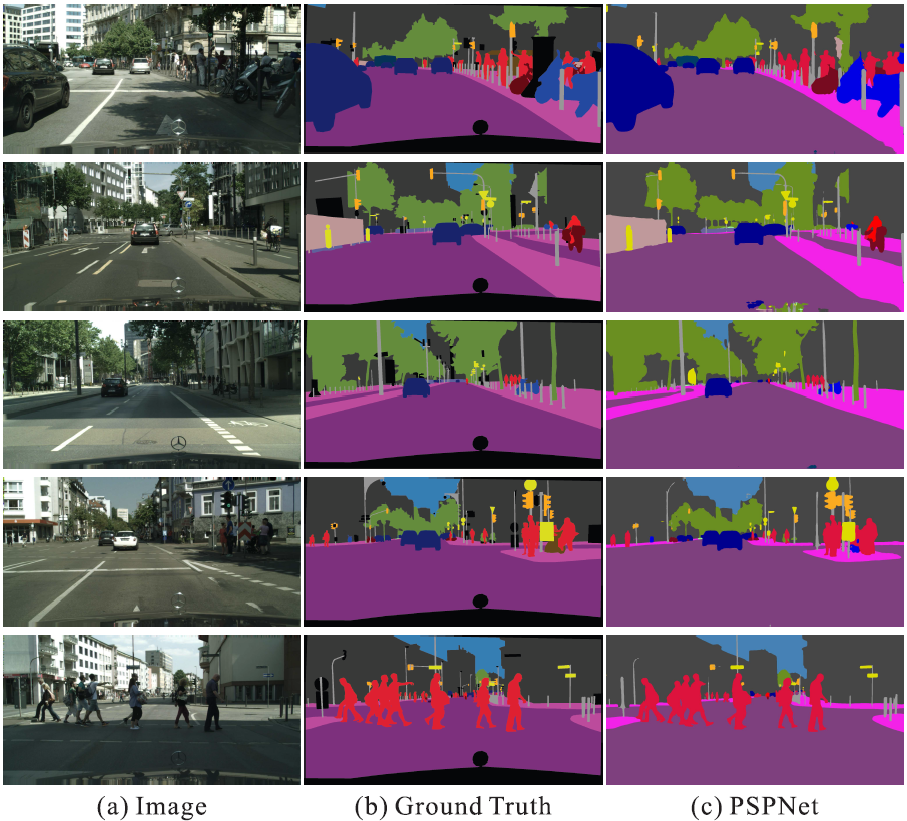
\includegraphics[width=5cm]{plots/cityscapes_visual.png}
    \caption{Given an input image, first CNN is used to get the feature map of the last convolutional layer, then a pyramid parsing module is applied to harvest different sub-region representations, followed by upsampling and concatenation layers to form the final feature representation, which carries both local and global context information. Finally, the representation is fed into a convolution layer to get the final per-pixel prediction. (Source: pyramid scene parsing network,by Zhao et. al, CVPR 2017) }
  \end{figure}
\framebreak
  \begin{figure}
    \centering
    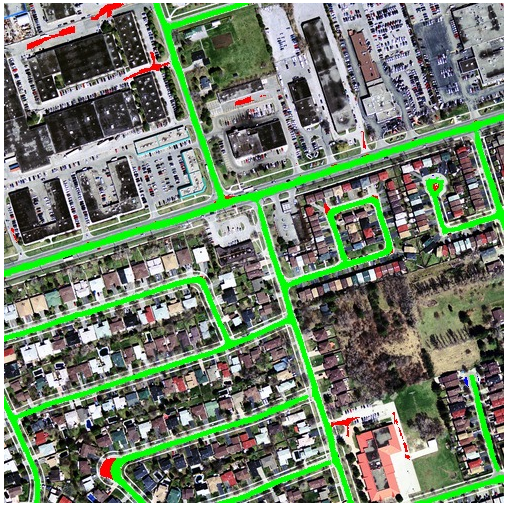
\includegraphics[width=6cm]{plots/01_introduction/road_seg.png}
    \caption{Road segmentation (Mnih Volodymyr (2013)). Aerial images and possibly outdated map pixels are labeled.}
  \end{figure}
\framebreak
\begin{wrapfigure}{R}{0.5\textwidth}
  \centering
  \scalebox{0.5}{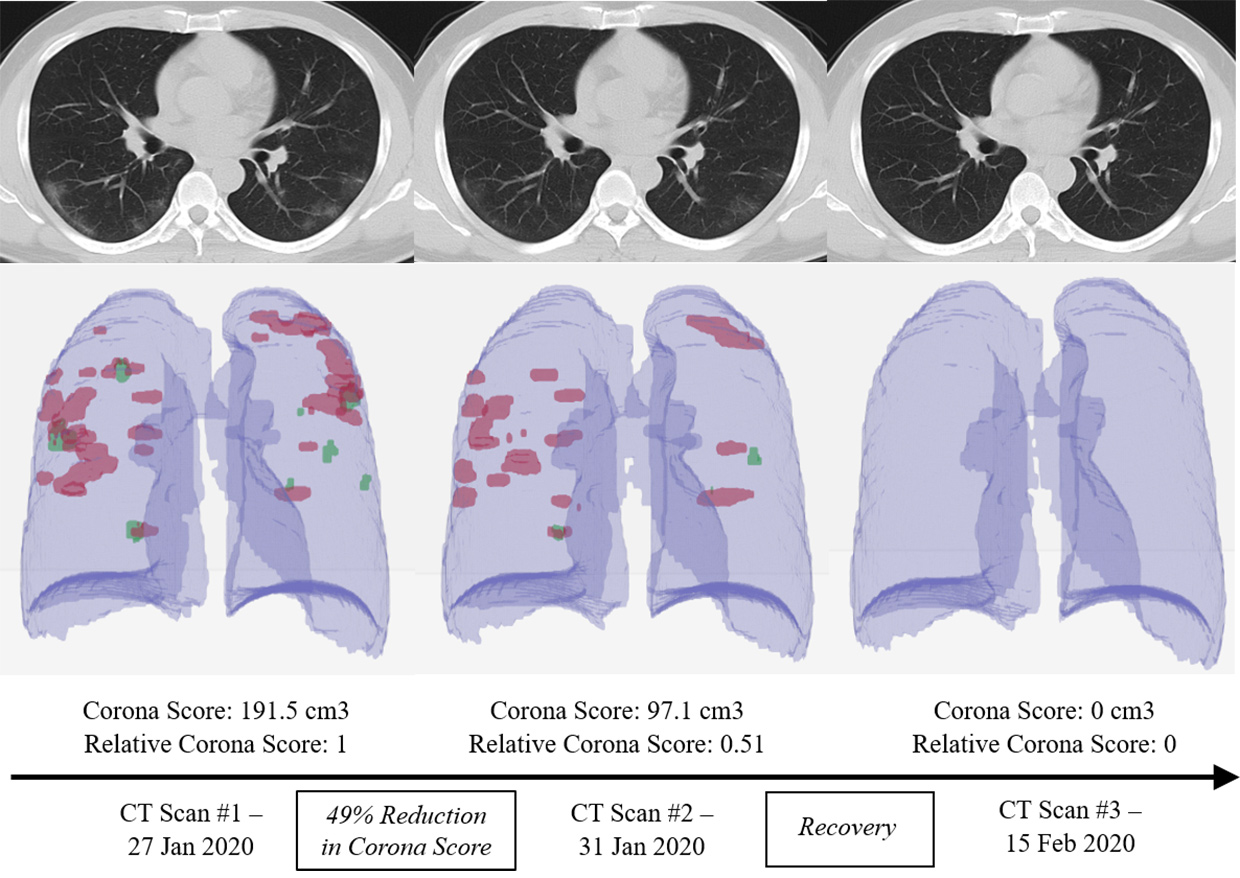
\includegraphics{plots/coronatrack.jpeg}}
\end{wrapfigure}

{CNN for personalized medicine: tracking, diagnosis and localization of Covid-19 patient}
  \begin{itemize}
    \item CNN based model (RADLogists) for personalized Covid-19 detection: three CT scans from a single coronavirus patient diagnosed by RADLogists 
  \end{itemize}
  
   \begin{figure}
    \centering
    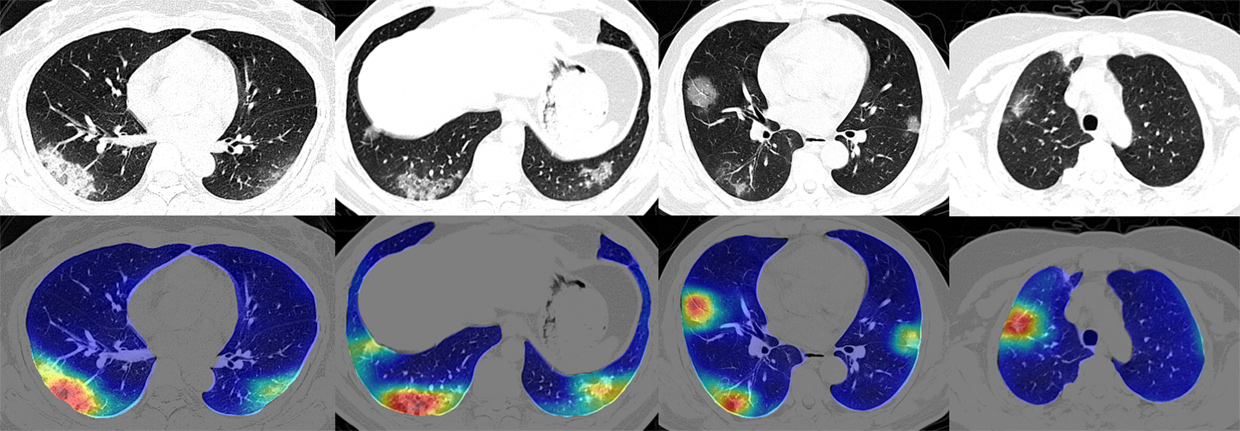
\includegraphics[width=6cm]{plots/hitmap.jpeg}
    \caption{Four COVID-19 lung CT scans (top) with corresponding colored maps showing coronavirus abnormalities (bottom).(source: IEEE Spectrum)}
  \end{figure}
\framebreak
  \begin{figure}
    \centering
    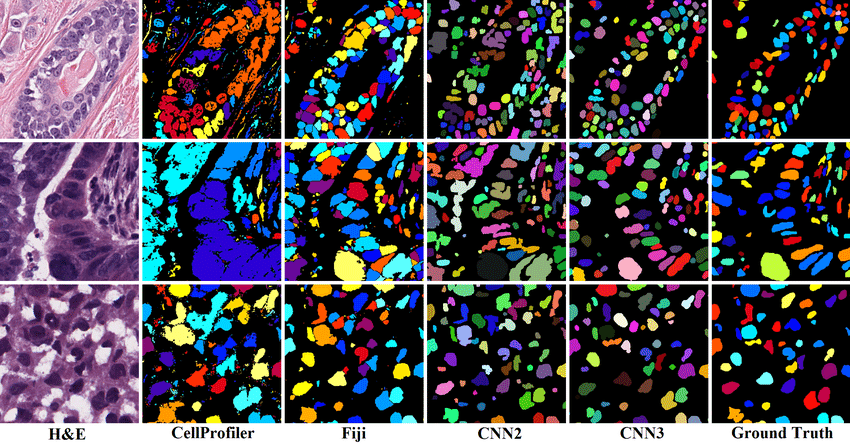
\includegraphics[width=9cm]{plots/instanceseg.png}
    \caption{Nuclear segmentation in digital microscopic tissue images can enable extraction of high-quality features for nuclear morphometrics and other analysis in computational pathology. (source: Kummar et. al. IEEE Transaction Medical Imaging) }
  \end{figure}
\framebreak
  \begin{figure}
    \centering
    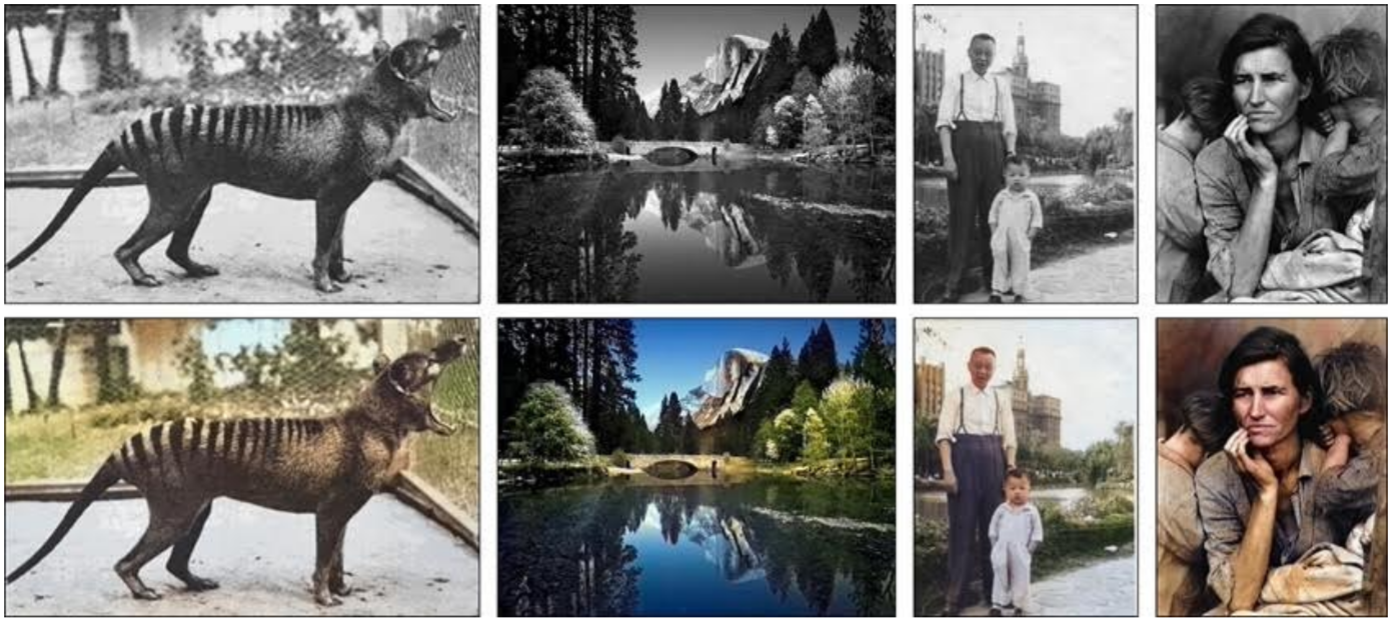
\includegraphics[width=11cm]{plots/01_introduction/colorization.png}
    \caption{Colorful Image Colorization (Zhang et al. (2016)). Given a grayscale photograph as input (top row), this network attacks the problem of hallucinating a plausible color version of the photograph (bottom row, i.e. the prediction of the network). Realizing this task manually consumes many hours of time.}
  \end{figure}
\framebreak
  \begin{figure}
    \centering
    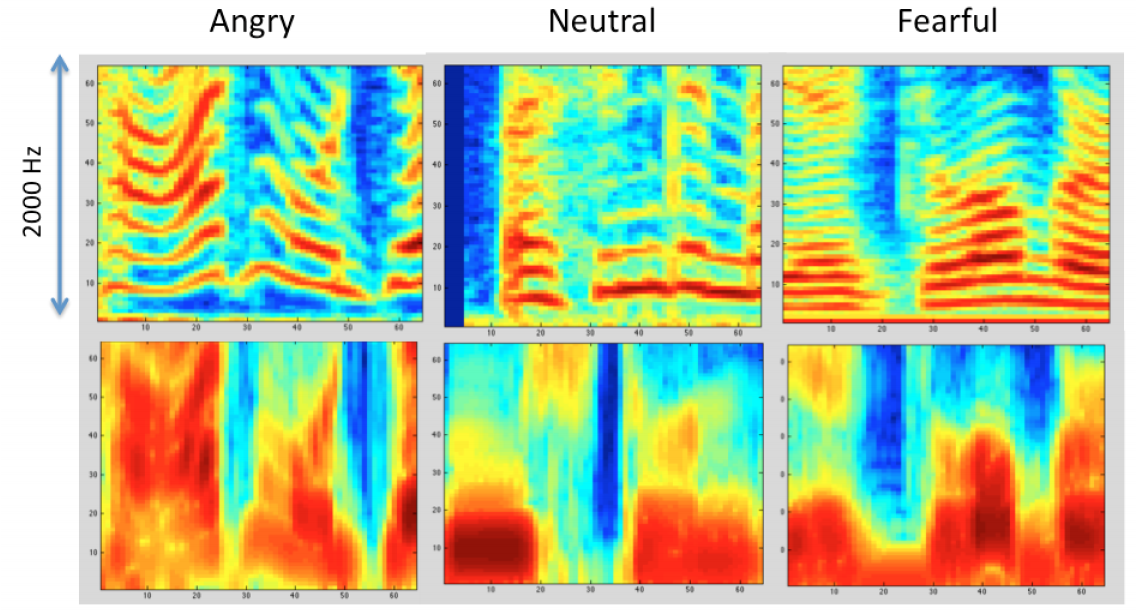
\includegraphics[width=10cm]{plots/01_introduction/speech.png}
    \caption{Speech recognition (Anand \& Verma (2015)). Convolutional neural network to extract features from audio data in order to classify emotions.}
  \end{figure}
\end{vbframe}
%%%%%%%%%%%%%%%%%%%%%%%%%%%%%%%%%%%%%%%%%%%%%%%%%%%%%%%%%%%%%%%%%%
%%%%%%%%%%%%%%%%%%%%%%%%%%%%%%%%%%%%%%%%%%%%%%%%%%%%%%%%%%%%%%%%%%
\frame{
\frametitle{CNNs - A First Glimpse}
 \center
    \only<1>{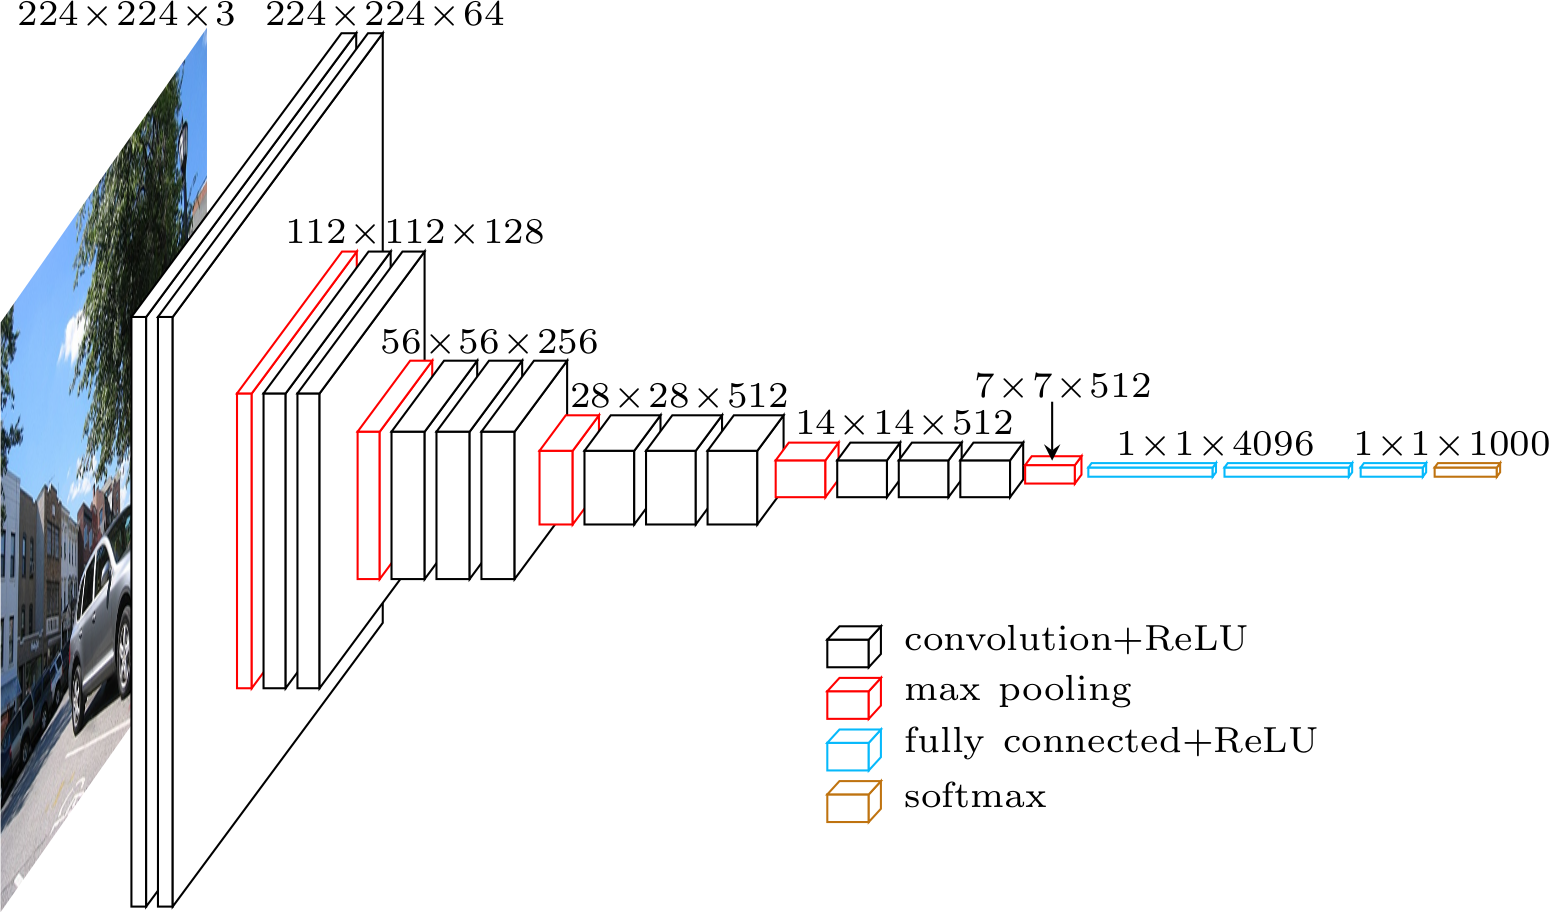
\includegraphics[width=9cm]{plots/01_introduction/alexnet.png}}%
    \only<2>{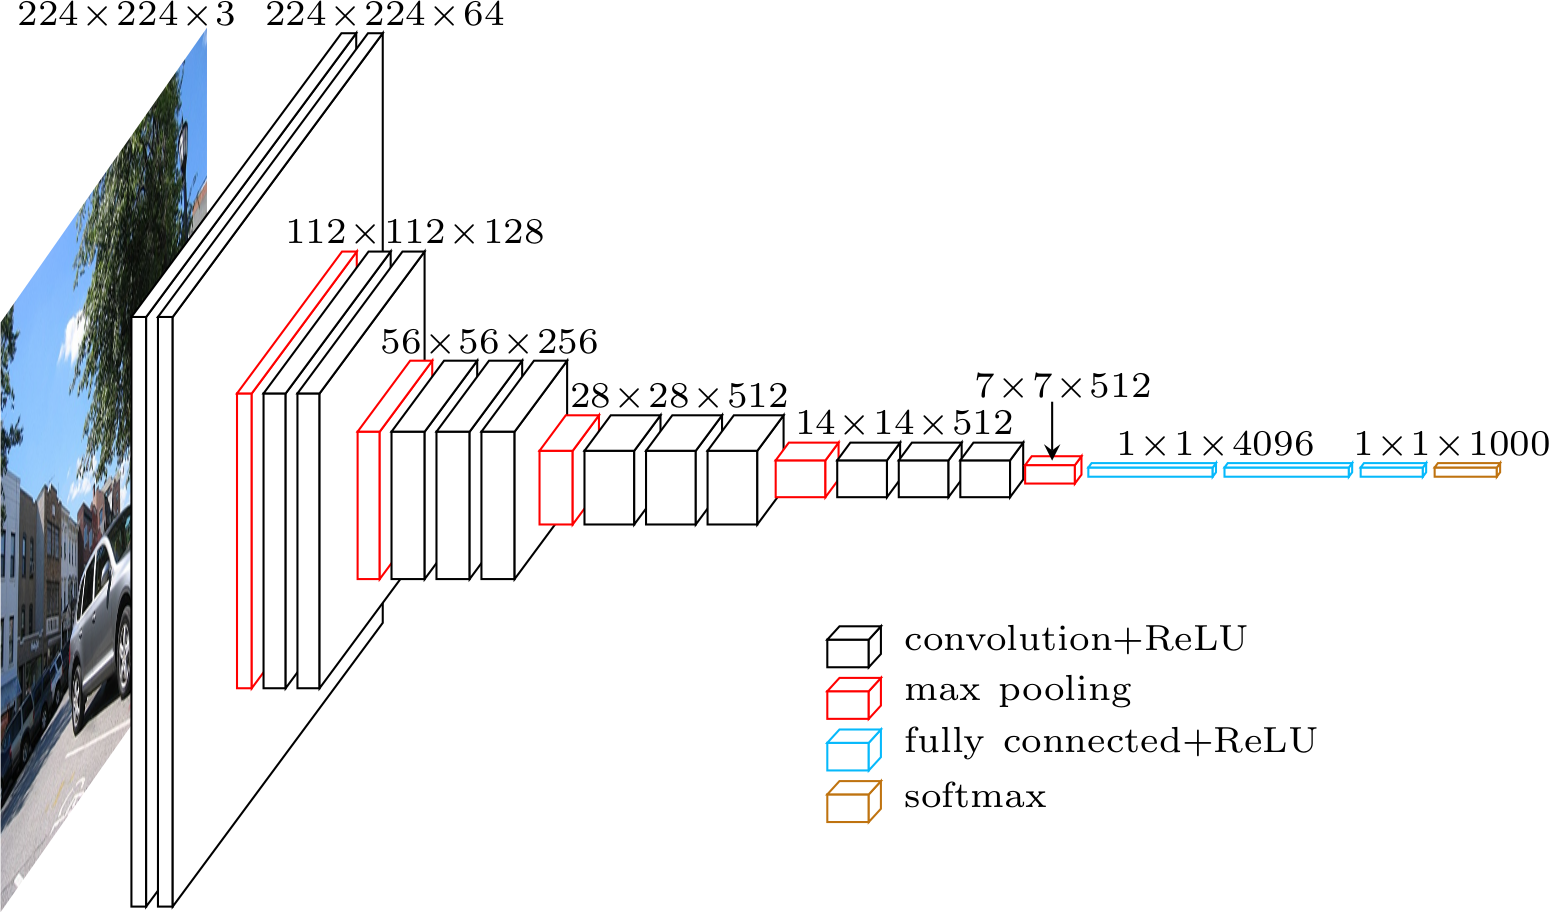
\includegraphics[width=9cm]{plots/01_introduction/alexnet.png}}%
    \begin{itemize}
        \only<1>{\item Input layer: contains the input (-image) as data matrices.}
        \only<1>{\item \textbf{Convolutions}: extract feature maps from a previous layer.}
        \only<1>{\item \textbf{Pooling}: reduces the dimensionality of any input and filter robust features.}
        \only<2>{\item Fully connected layer: standard layer that connects feature map elements with the output neurons.}
        \only<2>{\item Softmax: squashes output values to probability scores.}
    \end{itemize}
}
%%%%%%%%%%%%%%%%%%%%%%%%%%%%%%%%%%%%%%%%%%%%%%%%%%%%%%%%%%%%%%%%%%
%%%%%%%%%%%%%%%%%%%%%%%%%%%%%%%%%%%%%%%%%%%%%%%%%%%%%%%%%%%%%%%%%%

\section{Convolutions --- Basic Idea}

\begin{vbframe}{Filters to extract features}
    \begin{itemize}
        \item Filters are widely applied in Computer Vision (CV) since the 70's.
        \item One prominent example: \textbf{Sobel-Filter}.
        \item Detects edges in images.
    \end{itemize}
    \begin{figure}
        \centering
        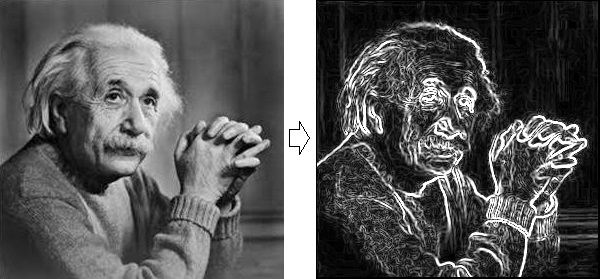
\includegraphics[width=10cm]{plots/02_filters/sobel_einstein.png}
        % source: https://github.com/qmegas/sobel-operator/blob/HEAD/images/1.jpg
        \caption{Sobel-filtered image.}
    \end{figure}
\framebreak
    \begin{itemize}
        \item Edges occur where the intensity over neighboring pixels changes fast.
        \item Thus, approximate the gradient of the intensity of each pixel.
        \item Sobel showed that the gradient image $G_x$ of original image $A$ in x-dimension  can be approximated by:
        $$
            G_x = 
            \begin{bmatrix}
                -1 & 0 & +1 \\
                -2 & 0 & +2 \\
                -1 & 0 & +1 
            \end{bmatrix} * A = S_x * A
        $$
        where $*$ indicates a mathematical operation known as a \textbf{convolution}, not a traditional matrix multiplication.
        \item The filter matrix $S_x$ consists of the product of an \textbf{averaging} and a \textbf{differentiation} kernel: 
        $$
            \underbrace{\begin{bmatrix}
                1 & 2 & 1   
            \end{bmatrix}^{T}}_{averaging}
        % $$
        % $$
            \underbrace{\begin{bmatrix}
                -1 & 0 & +1   
            \end{bmatrix}}_{differentiation}
        $$
        
        % \footnotesize{(Note :  More on this later.)}
    \end{itemize}
\framebreak
    \begin{itemize}
        \item Similarly, the gradient image $G_y$ in y-dimension can be approximated by:
        $$
            G_y = 
            \begin{bmatrix}
                -1 & -2 & -1  \\
                0 & 0 & 0 \\
                +1 & +2 & +1
            \end{bmatrix} * A = S_y * A
        $$
        \item The combination of both gradient images yields a dimension-independent gradient information $G$:
        $$
            G = \sqrt{G_x^2 + G_y^2}
        $$
        \item These matrix operations were used to create the filtered picture of Albert Einstein.
    \end{itemize}
\end{vbframe}

\begin{frame}{Horizontal vs Vertical edges}

    \begin{figure}
        \centering
          \scalebox{0.9}{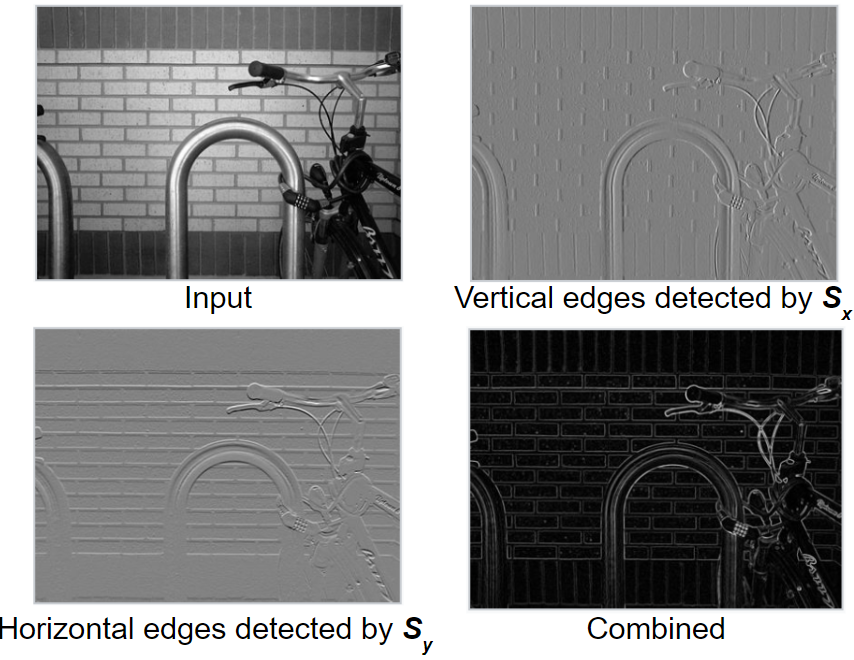
\includegraphics{plots/02_filters/sobel_bike.png}}
          \tiny{\\ Source: Wikipedia}
         \caption{\footnotesize{Sobel filtered images. Outputs are normalized in each case. }}
    \end{figure}

\end{frame}

\frame{
\frametitle{Filters to extract features}
    \center
    \only<1>{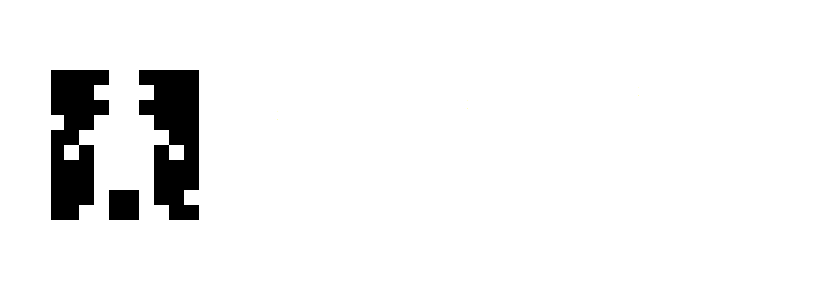
\includegraphics[width=11cm]{plots/02_filters/sobel1.png}}%
    \only<2>{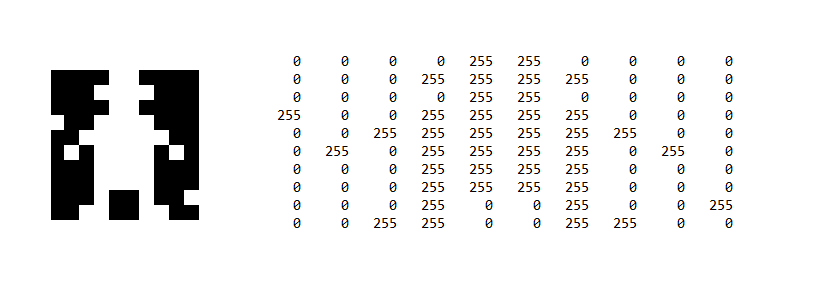
\includegraphics[width=11cm]{plots/02_filters/sobel2.png}}%
    \only<3>{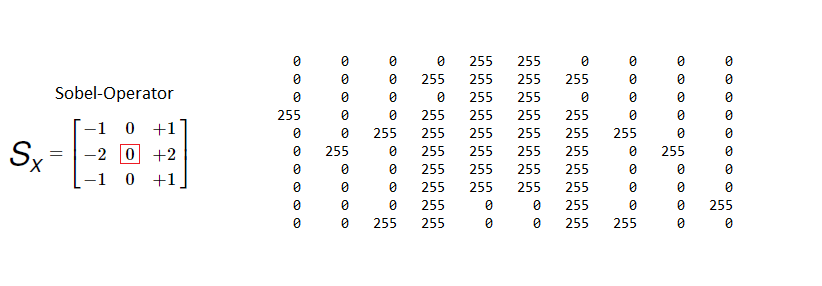
\includegraphics[width=11cm]{plots/02_filters/sobel3.png}}%
    \only<4>{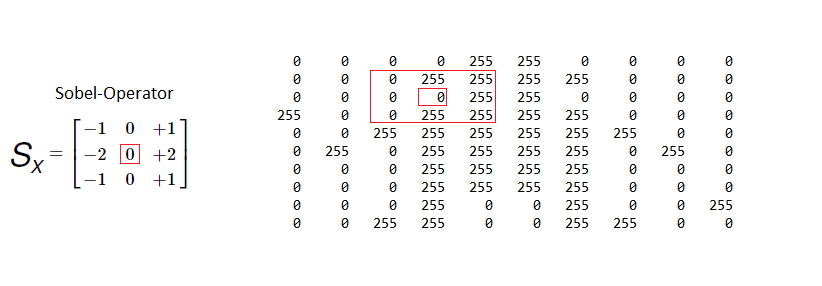
\includegraphics[width=11cm]{plots/02_filters/sobel4.png}}%
    \only<5>{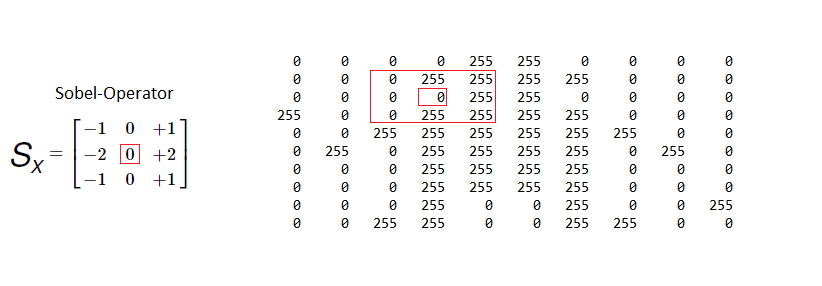
\includegraphics[width=11cm]{plots/02_filters/sobel4.png}}%
    %\only<6>{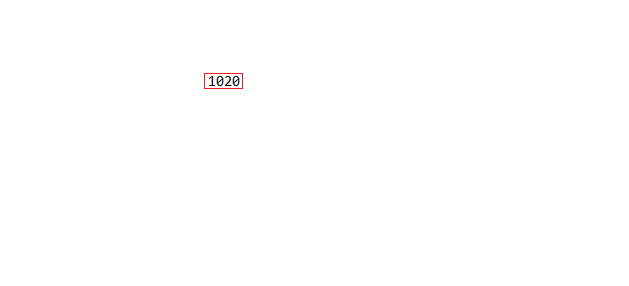
\includegraphics[width=11cm]{plots/02_filters/sobel5.png}}%
    \only<6>{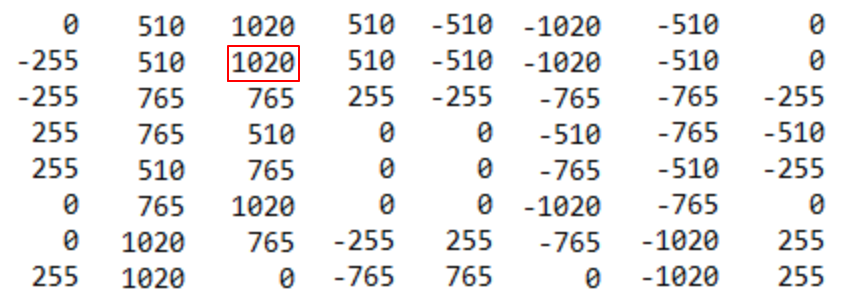
\includegraphics[width=6cm]{plots/02_filters/sobel6.png}}%
    \only<7>{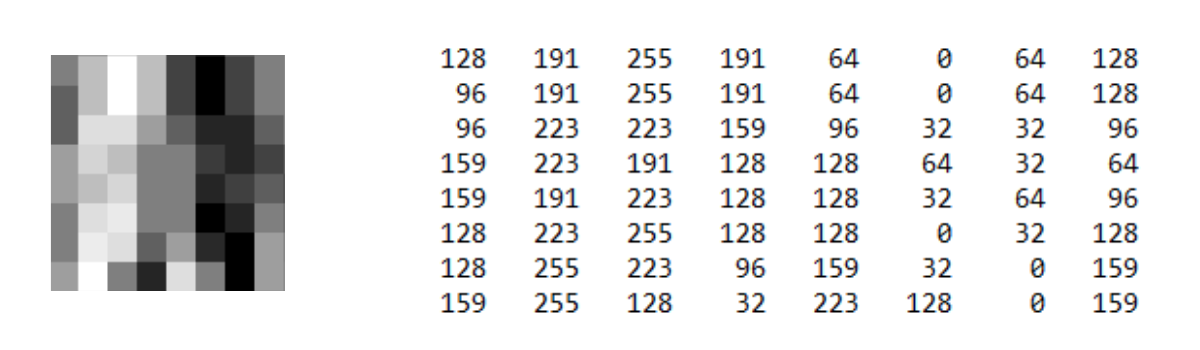
\includegraphics[width=11cm]{plots/02_filters/sobel8.png}}%

    \begin{itemize}
        \only<1>{\item Let's do this on a dummy image.}
        \only<1>{\item How to represent a digital image?}
        \only<2>{\item Basically as an array of integers.}
        \only<3>{\item $S_x$ enables us to to detect vertical edges!}
        \only<4>{\item[]}
        \only<5>{\item[]
        \vspace{-0.8cm}
        \begin{alignat*}{3}
            (\mathit{G}_x)_{(i,j)} = (I \star S_x)_{(i, j)}
                 & = -1 \cdot 0 \ \ &&+ \ \ 0 \cdot 255 \ \ &&+ \ \ \textbf{1} \cdot \textbf{255} \\
                 &\quad - 2 \cdot 0 &&+ \ \ 0 \cdot 0 &&+ \ \ \textbf{2} \cdot \textbf{255} \\
                 &\quad - 1 \cdot 0 &&+ \ \ 0 \cdot 255 &&+ \ \ \textbf{1} \cdot \textbf{255}
                 \notag
        \end{alignat*}
        }
        % \only<6>{\item[] \textcolor{white}{Applying the Sobel-Operator to every location in the input yields us the \textbf{feature map}.}}
        \only<6>{\item Applying the Sobel-Operator to every location in the input yields us the \textbf{feature map}.}
        \only<7>{\item Normalized feature map reveals vertical edges.
        \item Note the dimensional reduction compared to the dummy image.}
    \end{itemize}
}
%%%%%%%%%%%%%%%%%%%%%%%%%%%%%%%%%%%%%%%%%%%%%%%%%%%%%%%%%%%%%%%%%%
%%%%%%%%%%%%%%%%%%%%%%%%%%%%%%%%%%%%%%%%%%%%%%%%%%%%%%%%%%%%%%%%%%
\begin{vbframe}{Why do we need to know all of that?}
  \begin{itemize}
    \item What we just did was extracting \textbf{pre-defined} features from our input (i.e. edges).
    \item A convolutional neural network does almost exactly the same: \enquote{extracting features from the input}.
    \item[] $\Rightarrow$ The main difference is that we usually do not tell the CNN what to look for (pre-define them), \textbf{the CNN decides itself}.
    \item In a nutshell:
    \begin{itemize}
      \item We initialize a lot of random filters (like the Sobel but just random entries) and apply them to our input.
      \item Then, a classifier which is generally a feed forward neural net, uses them as input data.
      \item Filter entries will be adjusted by common gradient descent methods.
    \end{itemize}
  \end{itemize}
\end{vbframe}
%%%%%%%%%%%%%%%%%%%%%%%%%%%%%%%%%%%%%%%%%%%%%%%%%%%%%%%%%%%%%%%%%%
%%%%%%%%%%%%%%%%%%%%%%%%%%%%%%%%%%%%%%%%%%%%%%%%%%%%%%%%%%%%%%%%%%
\frame{

\frametitle{Why do we need to know all of that?}
    \center
    \only<1>{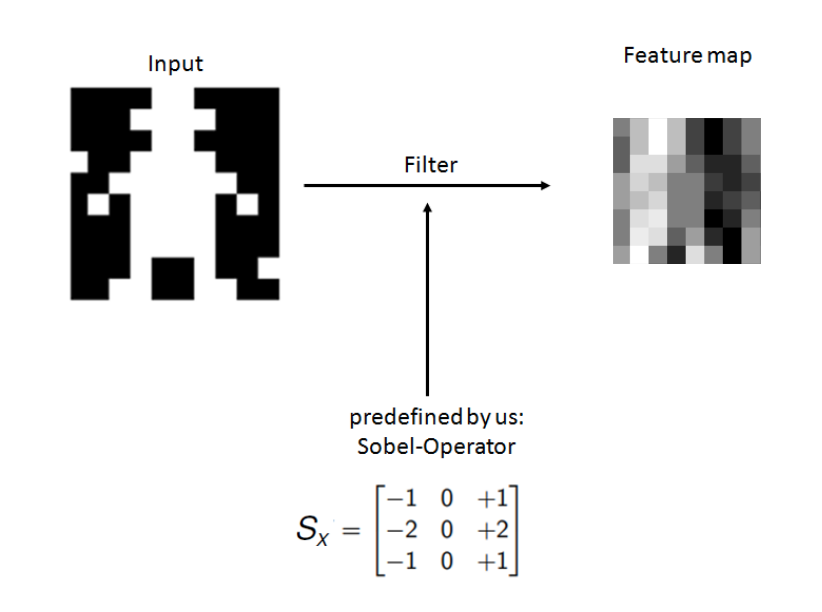
\includegraphics[width=11cm]{plots/02_filters/sobel9.png}}%
    \only<2>{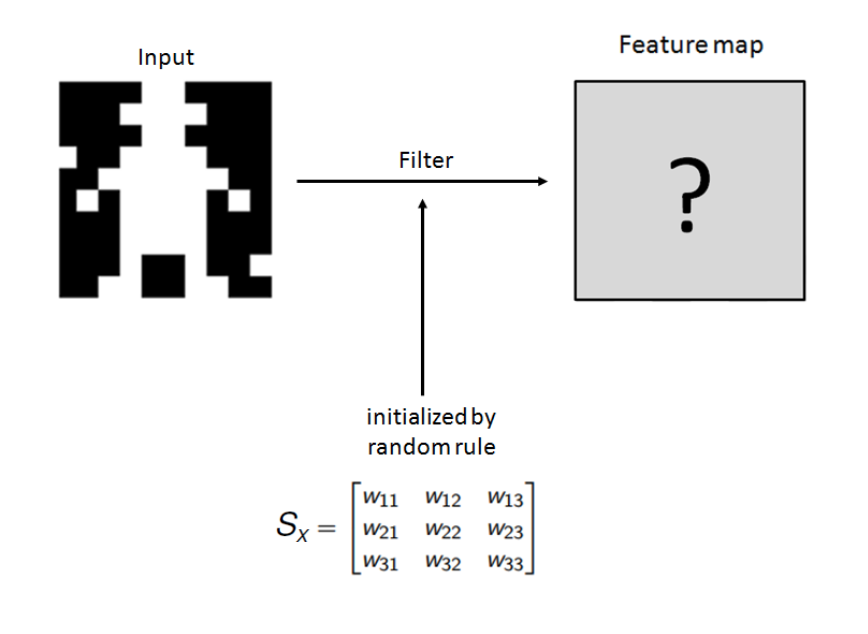
\includegraphics[width=10.5cm]{plots/02_filters/sobel10.png}}%
}
%%%%%%%%%%%%%%%%%%%%%%%%%%%%%%%%%%%%%%%%%%%%%%%%%%%%%%%%%%%%%%%%%%
%%%%%%%%%%%%%%%%%%%%%%%%%%%%%%%%%%%%%%%%%%%%%%%%%%%%%%%%%%%%%%%%%%
\begin{frame}{Working with images}
  \begin{itemize}
  \item In order to understand the functionality of CNNs, we have to familiarize ourselves with some properties of images.
  \item Grey scale images:
  \begin{itemize}
    \item Matrix with dimensions \textbf{h}eight $\times$ \textbf{w}idth $\times$ 1.
    \item Pixel entries differ from 0 (black) to 255 (white).
  \end{itemize}
  \item Color images:
  \begin{itemize}
    \item Tensor with dimensions \textbf{h}eight $\times$ \textbf{w}idth $\times$ 3.
    \item The depth 3 denotes the RGB values (red - green - blue).
  \end{itemize}
  \item Filters:
  \begin{itemize}
    \item A filter's depth is \textbf{always} equal to the input's depth!
    \item In practice, filters are usually square.
    \item Thus we only need one integer to define its size.
    \item For example, a filter of size $2$ applied on a color image actually has the dimensions $2 \times 2 \times 3$.
  \end{itemize}
  \end{itemize}
\end{frame}
%%%%%%%%%%%%%%%%%%%%%%%%%%%%%%%%%%%%%%%%%%%%%%%%%%%%%%%%%%%%%%%%%%
%%%%%%%%%%%%%%%%%%%%%%%%%%%%%%%%%%%%%%%%%%%%%%%%%%%%%%%%%%%%%%%%%%
\frame{

\frametitle{The 2d convolution}

  \begin{itemize}

    \only<1-8>{\item Suppose we have an input with entries $a, b, \dots, i$ (think of pixel values).}
    \only<1-8>{\item The filter we would like to apply has weights $w_{11}, w_{12}, w_{21} \text{ and } w_{22}$.}

  \end{itemize}

  \center
  \only<1>{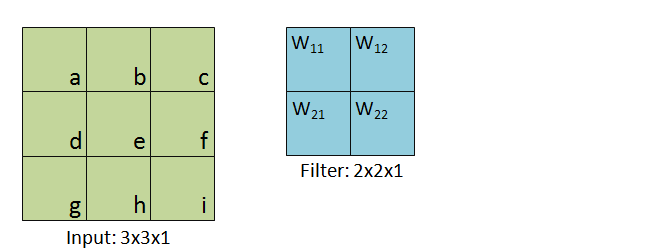
\includegraphics[width=8cm]{plots/04_conv2d/2dconv1.png}}%
  \only<2>{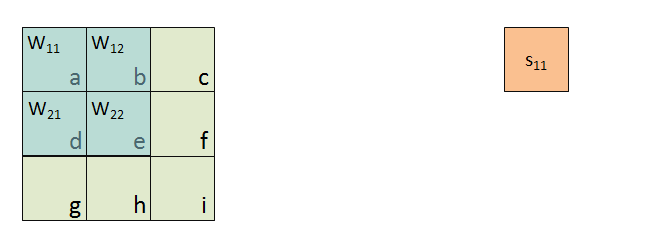
\includegraphics[width=8cm]{plots/04_conv2d/2dconv2.png}}%
  \only<3>{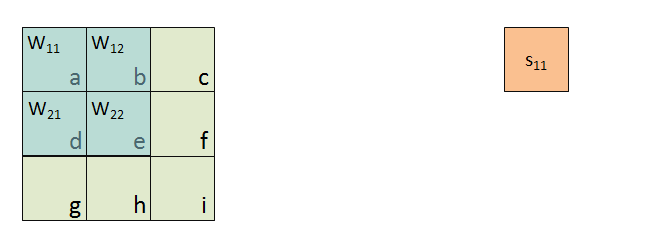
\includegraphics[width=8cm]{plots/04_conv2d/2dconv2.png}}%
  \only<4>{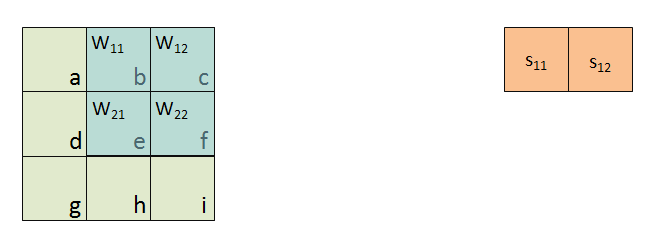
\includegraphics[width=8cm]{plots/04_conv2d/2dconv3.png}}%
  \only<5>{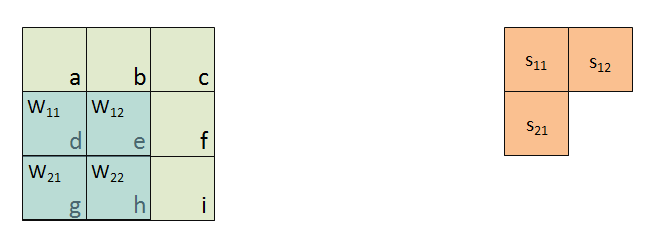
\includegraphics[width=8cm]{plots/04_conv2d/2dconv4.png}}%
  \only<6>{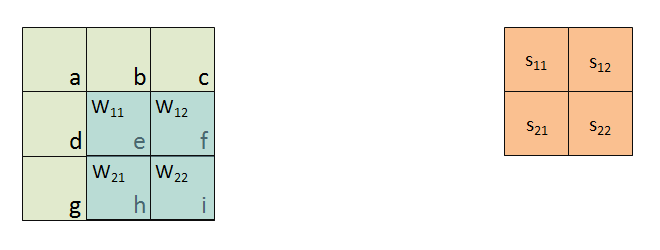
\includegraphics[width=8cm]{plots/04_conv2d/2dconv5.png}}%
  \only<7>{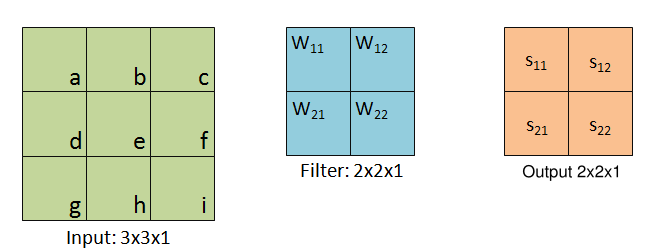
\includegraphics[width=8cm]{plots/04_conv2d/2dconv6.png}}%
  \only<8>{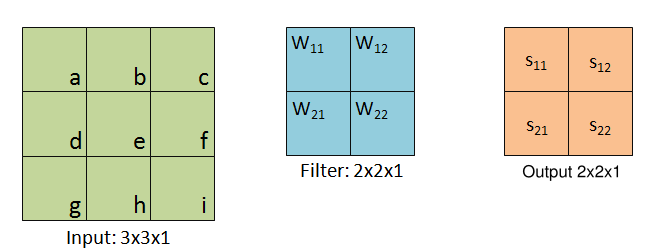
\includegraphics[width=8cm]{plots/04_conv2d/2dconv6.png}}%

  \begin{itemize}

    \only<1>{\item[] }
    \only<2>{\item[] }
    \only<3>{\item[] To obtain $s_{11}$ we simply compute the dot product:}
    \only<3>{\item[] $s_{11} = a \cdot w_{11} + b \cdot w_{12} + d \cdot w_{21} + e \cdot w_{22}$}
    \only<4>{\item[] Same for $s_{12}$:}
    \only<4>{\item[] $s_{12} = b \cdot w_{11} + c \cdot w_{12} + e \cdot w_{21} + f \cdot w_{22}$}
    \only<5>{\item[] As well as for $s_{21}$:}
    \only<5>{\item[] $s_{21} = d \cdot w_{11} + e \cdot w_{12} + g \cdot w_{21} + h \cdot w_{22}$}
    \only<6>{\item[] And finally for $s_{22}$:}
    \only<6>{\item[] $s_{22} = e \cdot w_{11} + f \cdot w_{12} + h \cdot w_{21} + i \cdot w_{22}$}
    \only<7>{\item[] $s_{11} = a \cdot w_{11} + b \cdot w_{12} + d \cdot w_{21} + e \cdot w_{22}$}
    \only<7>{\item[] $s_{12} = b \cdot w_{11} + c \cdot w_{12} + e \cdot w_{21} + f \cdot w_{22}$}
    \only<7>{\item[] $s_{21} = d \cdot w_{11} + e \cdot w_{12} + g \cdot w_{21} + h \cdot w_{22}$}
    \only<7>{\item[] $s_{22} = e \cdot w_{11} + f \cdot w_{12} + h \cdot w_{21} + i \cdot w_{22}$}
	\only<8>{\item[] More generally, let $I$ be the matrix representing the input and $W$ be the filter/kernel. Then the entries of the output matrix are defined by $s_{ij} = \sum_{m,n} I_{i+m-1, j+n-1} w_{mn}$ where $m,n$ denote the image size and kernel size respectively.}

  \end{itemize}

}

%%%%%%%%%%%%%%%%%%%%%%%%%%%%%%%%%%%%%%%%%%%%%%%%%%%%%%%%%%%%%%%%%%
%%%%%%%%%%%%%%%%%%%%%%%%%%%%%%%%%%%%%%%%%%%%%%%%%%%%%%%%%%%%%%%%%%
\section{Network properties induced by convolution}
%%%%%%%%%%%%%%%%%%%%%%%%%%%%%%%%%%%%%%%%%%%%%%%%%%%%%%%%%%%%%%%%%%

\frame{

\frametitle{Sparse interactions}

  \center
  \only<1>{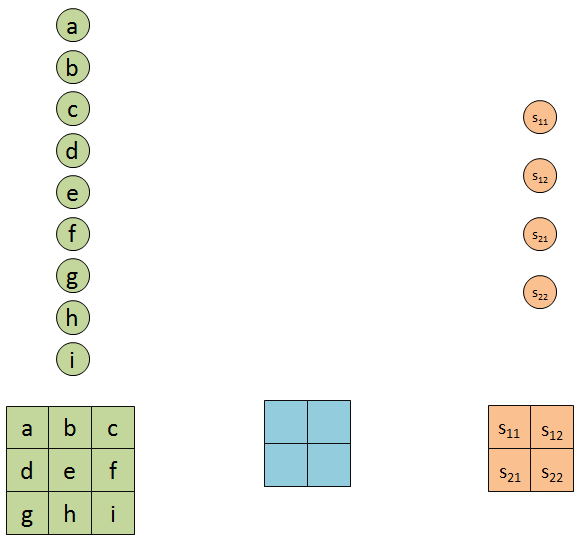
\includegraphics[width=7cm]{plots/06_conv_properties/sparse/sparse0.png}}%
  \only<2>{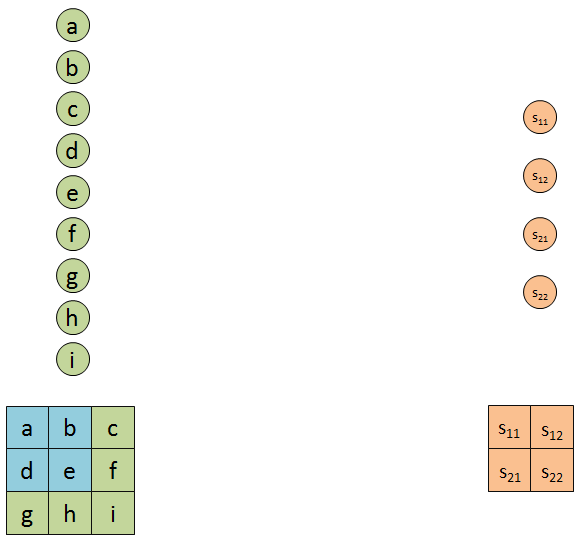
\includegraphics[width=7cm]{plots/06_conv_properties/sparse/sparse1.png}}%
  \only<3>{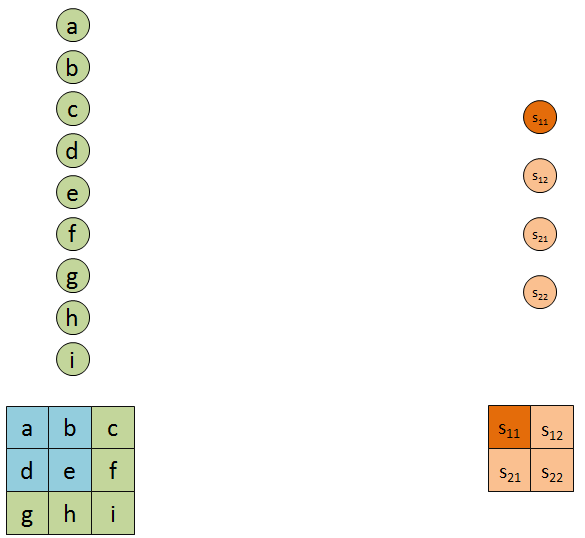
\includegraphics[width=7cm]{plots/06_conv_properties/sparse/sparse2.png}}%
  \only<4>{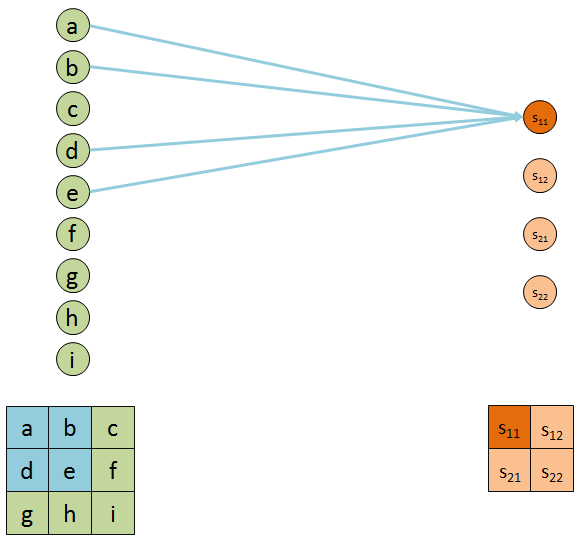
\includegraphics[width=7cm]{plots/06_conv_properties/sparse/sparse3.png}}%
  \only<5>{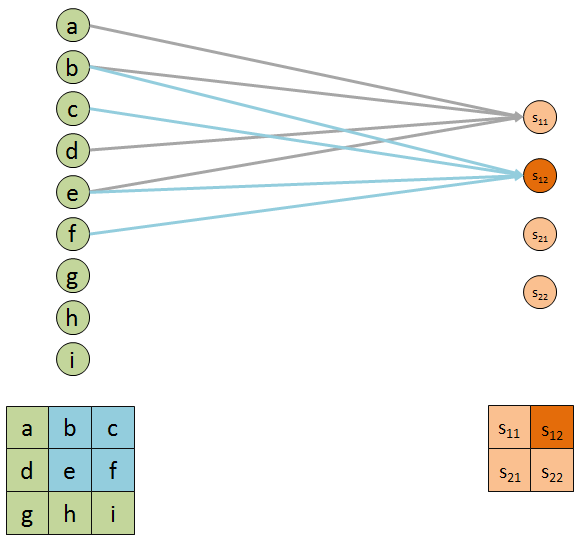
\includegraphics[width=7cm]{plots/06_conv_properties/sparse/sparse4.png}}%
  \only<6>{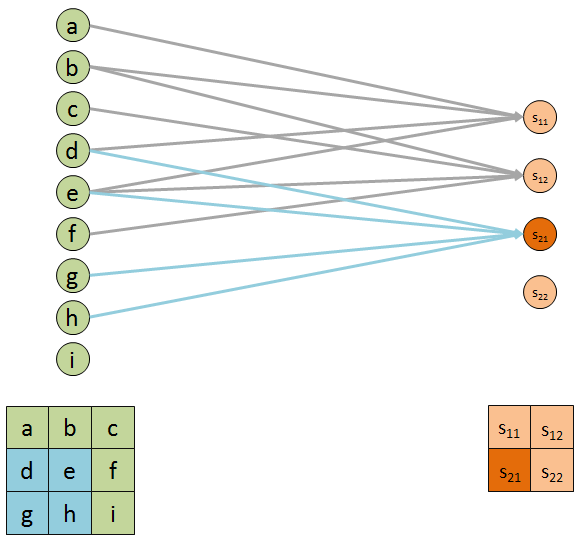
\includegraphics[width=7cm]{plots/06_conv_properties/sparse/sparse5.png}}%
  \only<7>{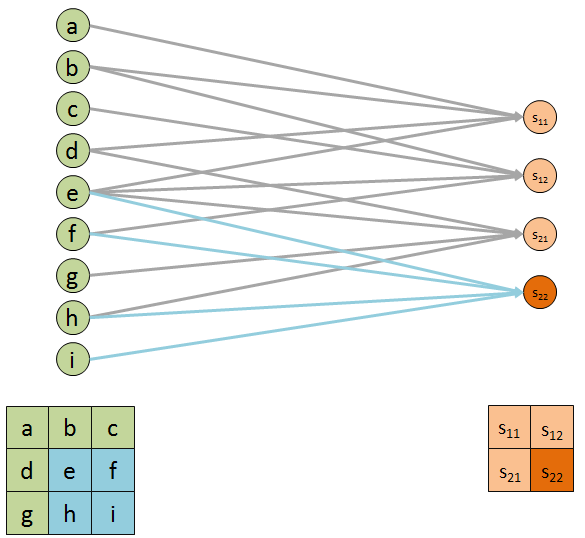
\includegraphics[width=7cm]{plots/06_conv_properties/sparse/sparse6.png}}%
  \only<8>{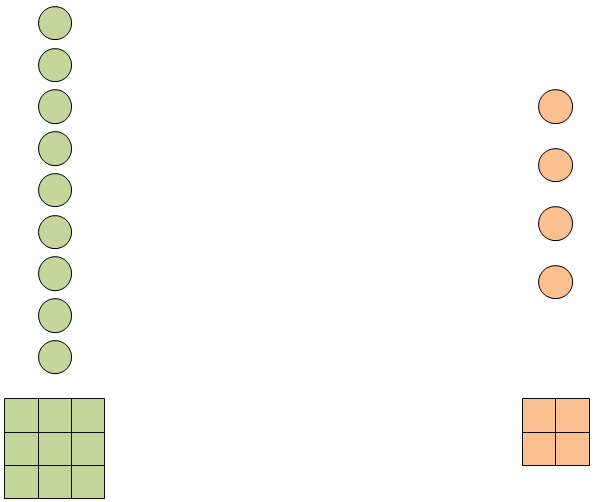
\includegraphics[width=7cm]{plots/06_conv_properties/sparse/dense0.png}}%
  \only<9>{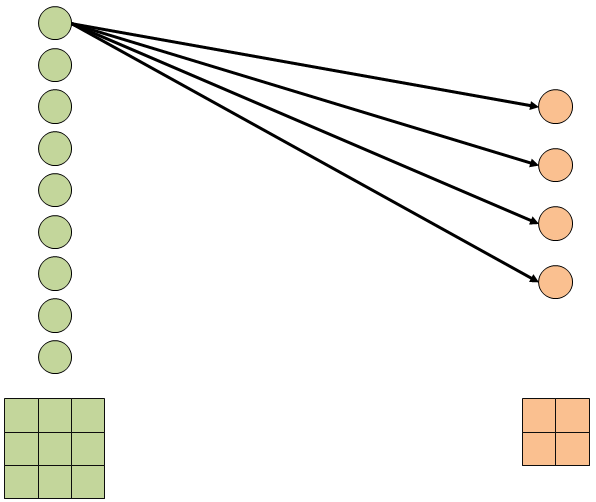
\includegraphics[width=7cm]{plots/06_conv_properties/sparse/dense1.png}}%
  \only<10>{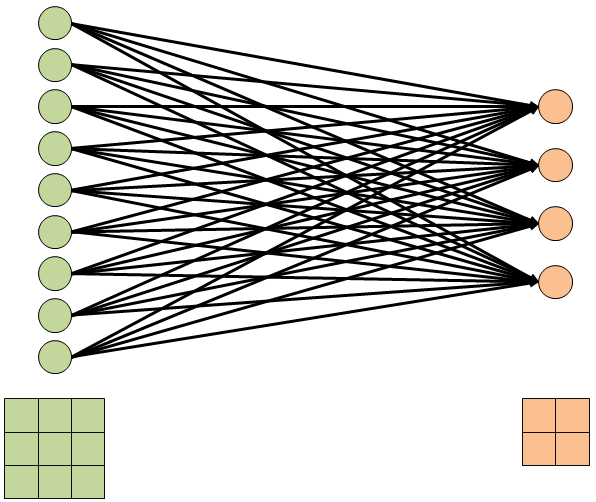
\includegraphics[width=7cm]{plots/06_conv_properties/sparse/dense2.png}}%

  \begin{itemize}

    \only<1>{\item We want to use the \enquote{neuron-wise} representation of our CNN.}
    \only<2>{\item Moving the filter to the first spatial location...}
    \only<3>{\item ...yields us the first entry of the feature map...}
    \only<4>{\item ...which is composed of these four connections.}
    \only<5>{\item $s_{12}$ is composed by these four connections.}
    \only<6>{\item $s_{21}$ by these..}
    \only<7>{\item and finally $s_{22}$ by these.}
    \only<8>{\item Assume we would replicate the architecture with a dense net.}
    \only<9>{\item Each input neuron is connected with each hidden layer neuron.}
    \only<10>{\item In total, we obtain 36 connections!}

  \end{itemize}

}
%%%%%%%%%%%%%%%%%%%%%%%%%%%%%%%%%%%%%%%%%%%%%%%%%%%%%%%%%%%%%%%%%%
%%%%%%%%%%%%%%%%%%%%%%%%%%%%%%%%%%%%%%%%%%%%%%%%%%%%%%%%%%%%%%%%%%
\begin{frame}{Sparse interactions}
  \begin{itemize}
    \item What does that mean?
    \begin{itemize}
      \item Our CNN has a \textbf{receptive field} of 4 neurons.
      \item That means, we apply a \enquote{local search} for features.
      \item A dense net on the other hand conducts a \enquote{global search}.
      \item The receptive field of the dense net are 9 neurons.
    \end{itemize}
    \item When processing images, it is more likely that features occur at specific locations in the input space.
    \item For example, it is more likely to find the eyes of a human in a certain area, like the face.
    \begin{itemize}
      \item A CNN only incorporates the surrounding area of the filter into its feature extraction process.
      \item The dense architecture on the other hand assumes that every single pixel entry has an influence on the eye, even pixels far away or in the background.
    \end{itemize}
  \end{itemize}
\end{frame}
%%%%%%%%%%%%%%%%%%%%%%%%%%%%%%%%%%%%%%%%%%%%%%%%%%%%%%%%%%%%%%%%%%
%%%%%%%%%%%%%%%%%%%%%%%%%%%%%%%%%%%%%%%%%%%%%%%%%%%%%%%%%%%%%%%%%%

\frame{

\frametitle{Parameter Sharing}

  \center
  \only<1>{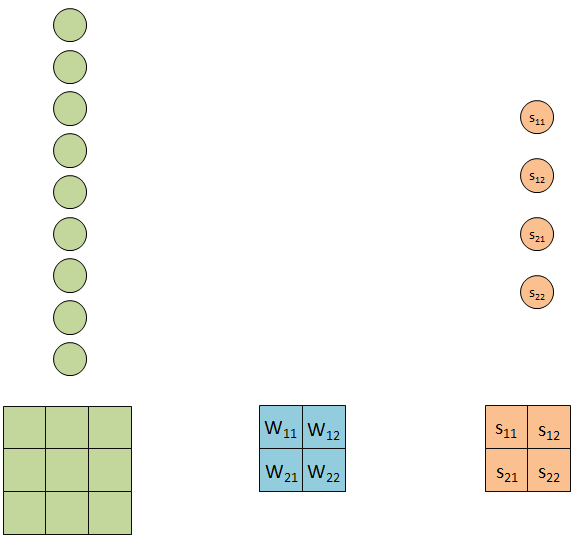
\includegraphics[width=7cm]{plots/06_conv_properties/ps/ps0.png}}%
  \only<2>{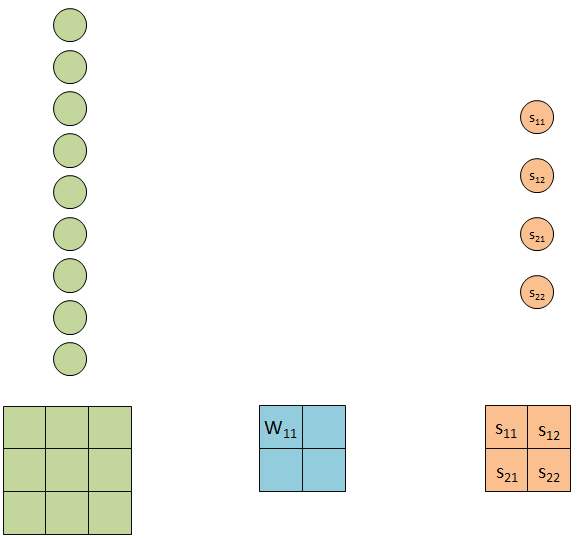
\includegraphics[width=7cm]{plots/06_conv_properties/ps/ps1.png}}%
  \only<3>{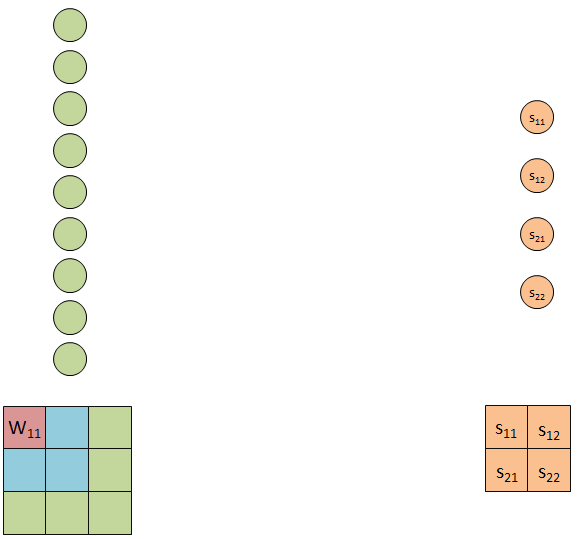
\includegraphics[width=7cm]{plots/06_conv_properties/ps/ps3.png}}%
  \only<4>{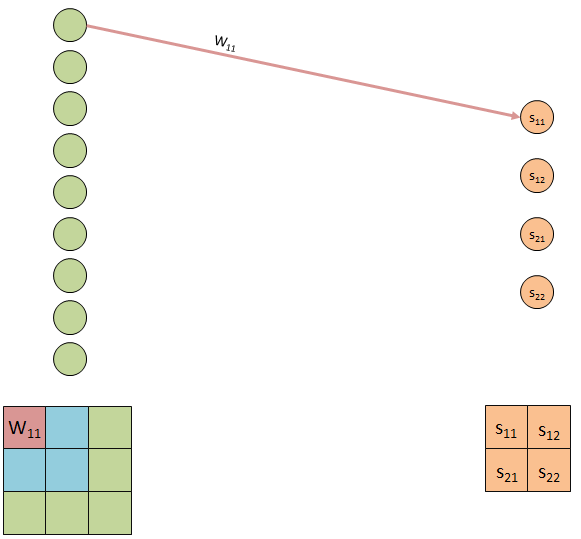
\includegraphics[width=7cm]{plots/06_conv_properties/ps/ps4.png}}%
  \only<5>{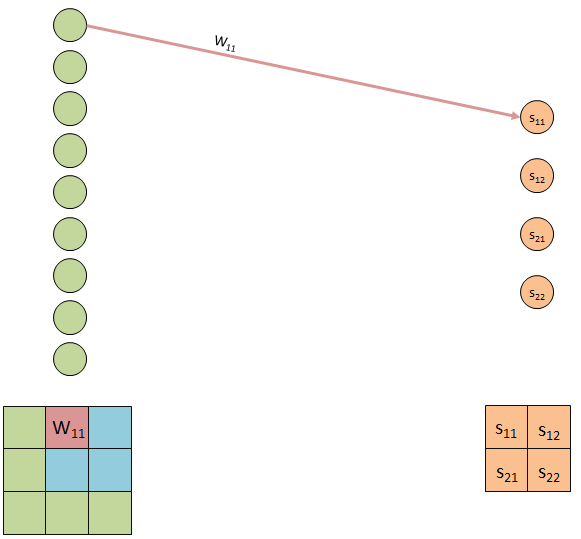
\includegraphics[width=7cm]{plots/06_conv_properties/ps/ps5.png}}%
  \only<6>{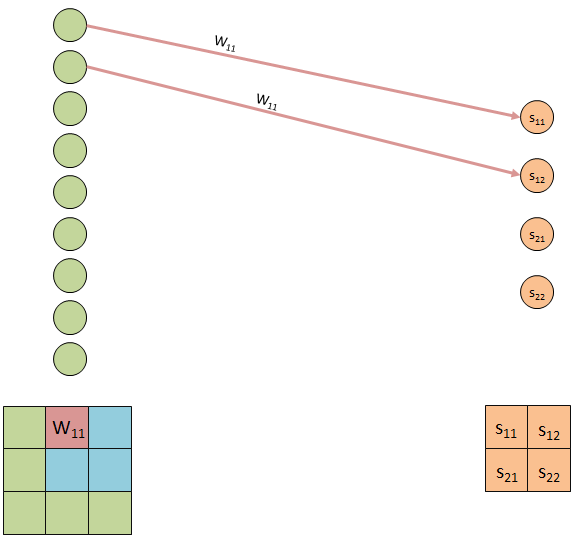
\includegraphics[width=7cm]{plots/06_conv_properties/ps/ps6.png}}%
  \only<7>{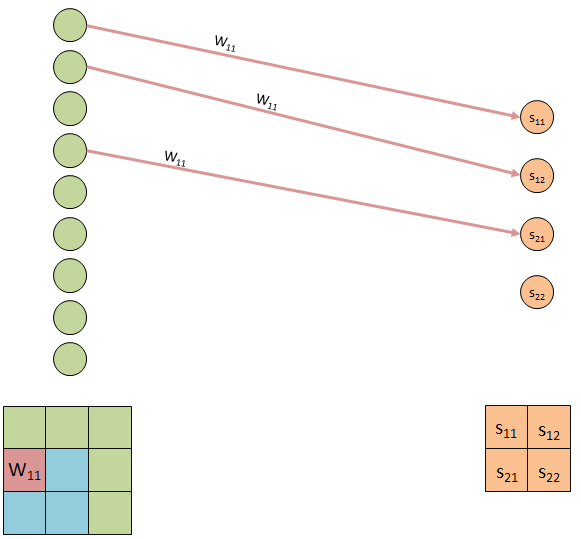
\includegraphics[width=7cm]{plots/06_conv_properties/ps/ps7.png}}%
  \only<8>{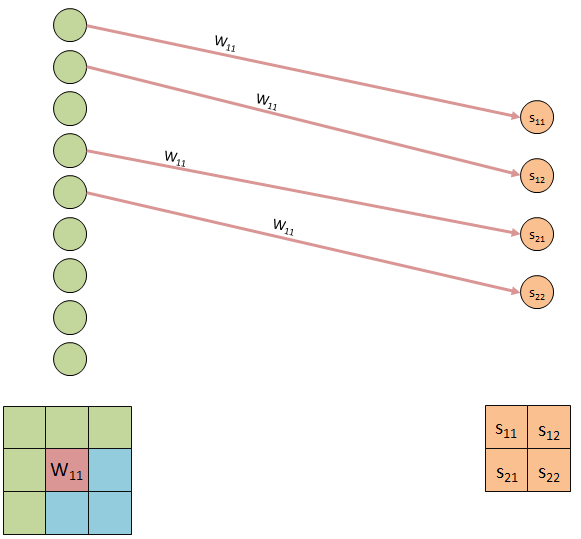
\includegraphics[width=7cm]{plots/06_conv_properties/ps/ps8.png}}%
  \only<9>{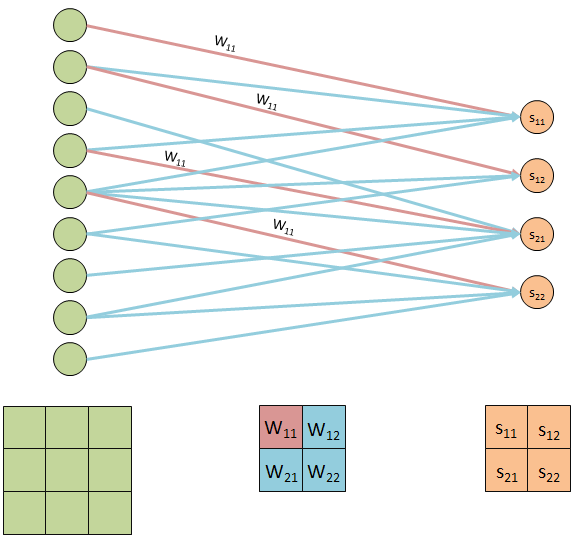
\includegraphics[width=7cm]{plots/06_conv_properties/ps/ps9.png}}%
  \only<10>{\includegraphics[width=7cm]{plots/06_conv_properties/ps/dense0.png}}%
  \only<11>{\includegraphics[width=7cm]{plots/06_conv_properties/ps/dense1.png}}%

  \begin{itemize}

    \only<1>{\item For the next property we focus on the filter entries.}
    \only<2>{\item In particular, we consider weight $w_{11}$}
    \only<3>{\item As we move the filter to the first spatial location..}
    \only<4>{\item ...we observe the following connection for weight $w_{11}$}
    \only<5>{\item Moving to the next location...}
    \only<6>{\item ...highlights that we use the same weight more than once!}
    \only<7>{\item Even three...}
    \only<8>{\item And in total four times.}
    \only<9>{\item All together, we have just used four weights.}
    \only<10>{\item How many weights does a corresponding dense net use?}
    \only<11>{\item $9 \cdot 4 = 36$! That is 9 times more weights!}

  \end{itemize}

}
%%%%%%%%%%%%%%%%%%%%%%%%%%%%%%%%%%%%%%%%%%%%%%%%%%%%%%%%%%%%%%%%%%
%%%%%%%%%%%%%%%%%%%%%%%%%%%%%%%%%%%%%%%%%%%%%%%%%%%%%%%%%%%%%%%%%%
\begin{vbframe}{Sparse Connections and Parameter sharing}
  \begin{itemize}
    \item Why is that good?
    \item Less parameters drastically reduce memory requirements.
    \item Faster runtime:
    \begin{itemize}
      \item For $m$ inputs and $n$ outputs, a fully connected layer requires $m\times n$ parameters and has $\mathcal{O}(m\times n)$ runtime.
      \item A convolutional layer has limited connections $k<<m$, thus only $k\times n$ parameters and $\mathcal{O}(k\times n)$ runtime.
    \end{itemize}
    \item But it gets even better:
    \begin{itemize}
      \item Less parameters mean less overfitting and better generalization!
    \end{itemize}
  \end{itemize}
\framebreak
  \begin{itemize}
    \item Example: consider a color image with size $100 \times 100$.
    \item Suppose we would like to create one single feature map with a \enquote{same padding} (i.e. the hidden layer is of the same size).
    %(i.e. retain the dim of the input for our feature maps).
    \begin{itemize}
      \item Choosing a filter with size $5$ means that we have a total of $5 \cdot 5 \cdot 3 = 75$ parameters (bias unconsidered).
      \item A dense net with the same amount of \enquote{neurons} in the hidden layer results in 
      $$\underbrace{(100^2 \cdot 3)}_{\text{input}} \cdot \underbrace{(100^2)}_{\text{hidden layer}} = 300.000.000 $$ parameters.
      
      %\item A dense net needs $10.000$ neurons in its hidden layer to replicate that architecture ($100 \cdot 100 = 10.000$). It has $100 \cdot 100 \cdot 3 \cdot 10.000 = 300.000.000$ parameters (bias unconsidered)!
      
    \end{itemize}
  \item Note that this was just a fictitious example. In practice we do not try to replicate CNN architectures with dense networks (actually it isn't even possible since physical limitations like the computer hardware would not allow us to).
  \end{itemize}
\end{vbframe}
%%%%%%%%%%%%%%%%%%%%%%%%%%%%%%%%%%%%%%%%%%%%%%%%%%%%%%%%%%%%%%%%%%
%%%%%%%%%%%%%%%%%%%%%%%%%%%%%%%%%%%%%%%%%%%%%%%%%%%%%%%%%%%%%%%%%%

\frame{

\frametitle{Equivariance to translation}

  \center
  \only<1>{\includegraphics[width=7cm]{plots/06_conv_properties/equivariance/equi0.png}}%
  \only<2>{\includegraphics[width=7cm]{plots/06_conv_properties/equivariance/equi1.png}}%
  \only<3>{\includegraphics[width=7cm]{plots/06_conv_properties/equivariance/equi2.png}}%
  \only<4>{\includegraphics[width=7cm]{plots/06_conv_properties/equivariance/equi3.png}}%

  \begin{itemize}

    \only<1>{\item Think of a specific feature of interest, here highlighted in grey.}
    \only<2>{\item Furthermore, assume we had a tuned filter looking for exactly that feature.}
    \only<3>{\item The filter does not care at what location the feature of interest is located at.}
    \only<4>{\item It is literally able to find it anywhere! That property is called \textbf{equivariance to translation}. \\[0.2cm] \scriptsize{Note: A function $f(x)$ is equivariant to a function $g$ if $f(g(x)) = g(f(x))$.}}
  \end{itemize}

}

%%%%%%%%%%%%%%%%%%%%%%%%%%%%%%%%%%%%%%%%%%%%%%%%%%%%%%%%%%%%%%%%%%
%%%%%%%%%%%%%%%%%%%%%%%%%%%%%%%%%%%%%%%%%%%%%%%%%%%%%%%%%%%%%%%%%%
\begin{frame}{Nonlinearity in feature maps}
    \begin{itemize}
        \item As in dense nets, we use activation functions on all feature map entries to introduce nonlinearity in the net.
        \item Typically rectified linear units (ReLU) are used in CNNs:
            \begin{itemize}
                \item They reduce the danger of saturating gradients compared to sigmoid activations.
                \item They can lead to \textit{sparse activations}, as neurons $\leq 0$ are squashed to $0$ which increases computational speed.
            \end{itemize}
        \item As seen in the last chapter, many variants of ReLU (Leaky ReLU, ELU, PReLU, etc.) exist.
    \end{itemize}
\end{frame}


% %%%%%%%%%%%%%%%%%%%%%%%%%%%%%%%%%%%%%%%%%%%%%%%%%%%%%%%%%%%%%%%%%%
% \section{Convolutions --- Mathematical Perspective}
% %%%%%%%%%%%%%%%%%%%%%%%%%%%%%%%%%%%%%%%%%%%%%%%%%%%%%%%%%%%%%%%%%%
% \begin{vbframe}{Convolutions: A Deeper Look}
%     \begin{itemize}
%         \item CNNs borrow their name from a mathematical operation termed \textbf{convolution} that originates in Signal Processing.
%         \item Basic understanding of this concept and related operations improves the understanding of the CNN functionality.
%         \item Still, there are successful practitioners that never heard of these concepts.
%         \item The following should provide exactly this fundamental understanding of convolutions.
%     \end{itemize}
% \framebreak
%     \begin{itemize}
%         \item Definition: \\
%             \begin{equation*}
%                 \begin{split}
%                     h(i) &= (f \ast g)(i) = \int_{-\infty}^{\infty} f(x)g(i-x)dx \\
%                     \text{where } f(x)& \text{ input function} \\
%                     \text{and } g(x)& \text{ weighting function, kernel} \\
%                     \text{and } h(i)& \text{ output function, feature map elements} \\
%                     \text{for } f, g &\in \R^{d} \mapsto h \in \R^{d}
%                 \end{split}
%             \end{equation*}
%         \item Intuition 1: Weighted smoothing of $f(x)$ with weighting function $g(x)$. 
%         \item Intuition 2: Filter function $g(x)$ filters features $h(i)$ from input signal $f(x)$.
%     \end{itemize}
% \framebreak
%     \begin{itemize}
%         \item Discretization for $\R^1$: \\
%             \begin{equation*}
%                 \begin{split}
%                     h(i) &= (f \ast g)(i) = \sum_{x = -\infty}^{\infty} f(x)g(i-x)
%                 \end{split}
%             \end{equation*}
%         \item Discretization for 2D images:
%             \begin{itemize}
%                 \item $\mathcal{I} \in \R^2$ contains two dimensions
%                 \item Use 2D Kernel $\mathcal{G}$ to yield feature map $\mathcal{H}$:
%                 \begin{equation*}
%                     \begin{split}
%                         \mathcal{H}(i, j) &= (\mathcal{I} \ast \mathcal{G})(i, j) = \sum_{x} \sum_{y} \mathcal{I}(x, y) \mathcal{G}(i-x, j-y) \\
%                         \text{where } x, y &:= \text{indices $\mathcal{I}$ and $\mathcal{G}$} \\
%                         \text{and } i, j &:= \text{indices elements in } \mathcal{H} \\
%                         \end{split}
%                 \end{equation*}
%             \end{itemize}
%     \end{itemize}
% \end{vbframe}    
% 
% %%%%%%%%%%%%%%%%%%%%%%%%%%%%%%%%%%%%%%%%%%%%%%%%%%%%%%%%%%%%%%%%%%
% %%%%%%%%%%%%%%%%%%%%%%%%%%%%%%%%%%%%%%%%%%%%%%%%%%%%%%%%%%%%%%%%%%
% \begin{vbframe}{1D Convolution Animation}
%     \begin{figure}
%     \centering
%     \includegraphics[width=10cm]{plots/conv_animations/conv_static.png}
%     \end{figure}
%     \begin{equation*}
%         f(x)=
%         \begin{cases}
%             1, & \text{if } x\in [-1, 2]\\
%             0, & \text{otherwise}
%         \end{cases}
%         \qquad
%         g(x)=
%         \begin{cases}
%             1 - 0.2*|x|, & \text{if } x > 0\\
%             0, & \text{otherwise}
%         \end{cases}
%     \end{equation*}
% \end{vbframe}
% 
% \begin{vbframe}{1D Convolution Animation}
%     \begin{figure}
%     \centering
%     \includegraphics[width=10cm]{plots/conv_animations/conv_static.png}
%     \end{figure}
%     Kernel is flipped due to the negative iterator in $$h(i) = \sum_{x = -\infty}^{\infty} f(x)g(i-x)$$
% \end{vbframe}
% 
% % \frame{
% % \frametitle{1D Convolution Animation}
% %     \center
% %         \only<1>{\includegraphics[width=11cm]{plots/conv_animations/conv_anim_1.png}}%
% %         \only<2>{\includegraphics[width=11cm]{plots/conv_animations/conv_anim_2.png}}%
% %         \only<3>{\includegraphics[width=11cm]{plots/conv_animations/conv_anim_3.png}}%
% %         \only<4>{\includegraphics[width=11cm]{plots/conv_animations/conv_anim_4.png}}%
% %         \only<5>{\includegraphics[width=11cm]{plots/conv_animations/conv_anim_5.png}}%
% %         \only<6>{\includegraphics[width=11cm]{plots/conv_animations/conv_anim_6.png}}%
% %         \only<7>{\includegraphics[width=11cm]{plots/conv_animations/conv_anim_7.png}}%
% %         \only<8>{\includegraphics[width=11cm]{plots/conv_animations/conv_anim_8.png}}%
% %         \only<9>{\includegraphics[width=11cm]{plots/conv_animations/conv_anim_9.png}}%
% %         \only<10>{\includegraphics[width=11cm]{plots/conv_animations/conv_anim_10.png}}%
% %         \only<11>{\includegraphics[width=11cm]{plots/conv_animations/conv_anim_11.png}}%
% %         \only<12>{\includegraphics[width=11cm]{plots/conv_animations/conv_anim_12.png}}%
% %         \only<13>{\includegraphics[width=11cm]{plots/conv_animations/conv_anim_13.png}}%
% %         \only<14>{\includegraphics[width=11cm]{plots/conv_animations/conv_anim_14.png}}%
% %         \only<15>{\includegraphics[width=11cm]{plots/conv_animations/conv_anim_15.png}}%
% %         \only<16>{\includegraphics[width=11cm]{plots/conv_animations/conv_anim_16.png}}%
% %         \only<17>{\includegraphics[width=11cm]{plots/conv_animations/conv_anim_17.png}}%
% %         \only<18>{\includegraphics[width=11cm]{plots/conv_animations/conv_anim_18.png}}%
% %         \only<19>{\includegraphics[width=11cm]{plots/conv_animations/conv_anim_19.png}}%
% %         \only<20>{\includegraphics[width=11cm]{plots/conv_animations/conv_anim_20.png}}%
% %         \only<21>{\includegraphics[width=11cm]{plots/conv_animations/conv_anim_21.png}}%
% %         \only<22>{\includegraphics[width=11cm]{plots/conv_animations/conv_anim_22.png}}%
% %         \only<23>{\includegraphics[width=11cm]{plots/conv_animations/conv_anim_23.png}}%
% %         \only<24>{\includegraphics[width=11cm]{plots/conv_animations/conv_anim_24.png}}%
% %         \only<25>{\includegraphics[width=11cm]{plots/conv_animations/conv_anim_25.png}}%
% %         \only<26>{\includegraphics[width=11cm]{plots/conv_animations/conv_anim_26.png}}%
% %         \only<27>{\includegraphics[width=11cm]{plots/conv_animations/conv_anim_27.png}}%
% %         \only<28>{\includegraphics[width=11cm]{plots/conv_animations/conv_anim_28.png}}%
% %         \only<29>{\includegraphics[width=11cm]{plots/conv_animations/conv_anim_29.png}}%
% % }
% 
% 
% \frame{
% \frametitle{1D Convolution Animation}
%     \center
%         \only<1>{\includegraphics[width=11cm]{plots/conv_animations/conv_anim_3.png}}%
%         \only<2>{\includegraphics[width=11cm]{plots/conv_animations/conv_anim_10.png}}%
%         \only<3>{\includegraphics[width=11cm]{plots/conv_animations/conv_anim_15.png}}%
%         \only<4>{\includegraphics[width=11cm]{plots/conv_animations/conv_anim_19.png}}%
%         \only<5>{\includegraphics[width=11cm]{plots/conv_animations/conv_anim_24.png}}%
%         \only<6>{\includegraphics[width=11cm]{plots/conv_animations/conv_anim_28.png}}%
% }
% 
% %%%%%%%%%%%%%%%%%%%%%%%%%%%%%%%%%%%%%%%%%%%%%%%%%%%%%%%%%%%%%%%%%%
% %%%%%%%%%%%%%%%%%%%%%%%%%%%%%%%%%%%%%%%%%%%%%%%%%%%%%%%%%%%%%%%%%%
% \begin{vbframe}{Properties of the Convolution}
%     \begin{itemize}
%         \item Commutativity:
%         $$ f \ast g = g \ast f$$
%         \item Associativity:
%         $$ (f \ast g) \ast h = f \ast (g \ast h)$$
%         \item Distributivity:
%         $$ f \ast (g + h) = f\ast g + f \ast h$$ 
%         $$ \alpha (f \ast g) = (\alpha f) \ast g \text{ for scalar } \alpha$$ 
%         \item Differentiability:
%         $$ \frac{\partial (f\ast g)(x)}{\partial x_i} = \frac{\partial f(x)}{\partial x_i}\ast g(x) = \frac{\partial g(x)}{\partial x_i} \ast f(x)$$ \\
%         $ \rightarrow (f\ast g)(x)$ is as many times differentiable as the max of $g(x)$ and $f(x)$.
%     \end{itemize}
% \end{vbframe}
% %%%%%%%%%%%%%%%%%%%%%%%%%%%%%%%%%%%%%%%%%%%%%%%%%%%%%%%%%%%%%%%%%%
% %%%%%%%%%%%%%%%%%%%%%%%%%%%%%%%%%%%%%%%%%%%%%%%%%%%%%%%%%%%%%%%%%%
% 
% \begin{vbframe}{Related operations}
%     \begin{itemize}
%         \item Convolution is strongly related to two other mathematical operators:
%         \begin{enumerate}
%             \item Fourier transform via the Convolution Theorem
%             \item Cross-correlation
%         \end{enumerate}
%     \end{itemize}
% \end{vbframe}
% 
% % nice explanation here: https://www.quora.com/How-are-neural-networks-related-to-Fourier-transforms
% \begin{vbframe}{Convolution Theorem}
%     \begin{itemize}
%         \item  Fourier transform of the convolution of two functions can be expressed as the product of their Fourier transforms:
%         $$ 
%             \mathcal{F} \{ f\ast g\} = \mathcal{F} \{f\}\mathcal{F} \{g\}
%         $$
%         \item Transformation of a signal from time to frequency domain.
%         \item Convolution in the time domain is equivalent to multiplication in frequency domain.
%         \item The computationally fastest way to compute a convolution is therefore taking the Fourier inverse of the multiplication of the Fourier-transformed input and filter function:
%         $$
%             (f \ast g)(t) = \mathcal{F}^{-1}\{\mathcal{F} \{f(t)\} \mathcal{F} \{g(t)\}\}
%         $$
%     \end{itemize}
% \end{vbframe}
% 
% % \begin{vbframe}{Convolution Theorem - Proof}
% %     \begin{equation*}
% %         \begin{split}
% %             \widehat{(f \ast g)(t)} &= \int_{-\infty}^\infty exp(-2 \pi i \omega t) \Big[ \int_{-\infty}^\infty f(\tau) g(t-\tau)d\tau \Big] \\
% %             & = \int_{-\infty}^\infty \int_{-\infty}^\infty exp(-2 \pi i \omega t) f(\tau)g(t-\tau)d\tau dt \\
% %             & \overset{Fubini}{=} \int_{-\infty}^\infty \Big[ \int_{-\infty}^\infty exp(-2 \pi i \omega t) f(\tau) g(t-\tau ) dt  \Big] d\tau \\
% %             & \overset{f(\tau) \perp t}{=} \int_{-\infty}^\infty f(\tau) \Big[ \int_{-\infty}^\infty exp(-2 \pi i \omega t) g(t-\tau) dt \Big]d \tau \\
% %             & \overset{u = t - \tau}{=} \int_{-\infty}^\infty f(\tau) \Big[ \int_{-\infty}^\infty exp(-2\pi i \omega \tau) exp(-2 \pi i \omega u) g(u) du \Big] d\tau \\
% %             & = \int_{-\infty}^\infty exp(-2 \pi i \omega \tau) f(\tau) \Big[ \int_{-\infty}^\infty exp(-2 \pi i \omega u) g(u) du \Big] d \tau \\
% %             & \overset{Fubini}{=} ...
% %         \end{split}
% %     \end{equation*}
% % \end{vbframe}
% % 
% % \begin{vbframe}{Convolution Theorem - Proof}
% %     \begin{equation*}
% %         \begin{split}
% %             &... \int_{-\infty}^\infty exp(-2 \pi i \omega \tau) f(\tau) d\tau \int_{-\infty}^\infty exp(-2 \pi i \omega u) g(u) du \\
% %             &= \hat{f(t)}\hat{g(t)}
% %         \end{split}
% %     \end{equation*}
% % \end{vbframe}
% 
% %%%%%%%%%%%%%%%%%%%%%%%%%%%%%%%%%%%%%%%%%%%%%%%%%%%%%%%%%%%%%%%%%%
% %%%%%%%%%%%%%%%%%%%%%%%%%%%%%%%%%%%%%%%%%%%%%%%%%%%%%%%%%%%%%%%%%%
% % nice xcor vs conv video by caltech
% % https://www.youtube.com/watch?v=MQm6ZP1F6ms
% 
% \begin{vbframe}{Cross-correlation}
%     \begin{itemize}
%         \item Measurement for similarity of two functions $f(x), g(x)$.
%         \item More specifically, at which position are the two functions most similar to each other? Where does the pattern of $g(x)$ match $f(x)$ the best?
%         \item Intuition:
%         \begin{itemize}
%                 \item Slide with $g(x)$ over $f(x)$ and at each discrete step compute the sum of the product of their elements.
%                 \item When peaks of both functions are aligned, the product of high (positive or negative) values will lead to high sums.
%                 \item Thus, both functions are most similar at points with equal peaks.
%         \end{itemize}
%     \end{itemize}
% \framebreak
%     \begin{itemize}
%         \item Definition: \\
%             \begin{equation*}
%                 \begin{split}
%                     h(i) &= (f \star g)(i) = \int_{-\infty}^{\infty} f(x)g(i+x)dx \\
%                     \text{where } f(x)& \text{ input function} \\
%                     \text{and } g(x)& \text{ weighting function, kernel} \\
%                     \text{and } h(i)& \text{ output function, feature map elements} \\
%                     \text{for } f, g &\in \R^{d} \mapsto h \in \R^{d}
%                 \end{split}
%             \end{equation*}
%     \end{itemize}
% \framebreak 
%     \begin{itemize}
%         \item Discrete formulation:
%             \begin{equation*}
%                 h(i) = (f \star g)(i) = \sum_{x = -\infty}^{\infty} f(x)g(i+x)
%             \end{equation*}
%         \item Thus:
%             \begin{equation*}
%                     f(i) \star g(i) = f(-i) \ast g(i)
%             \end{equation*}
%         \item Remember: $\ast$ is used for convolution and $\star$ for cross-correlation.
%         \item Similar formulation as the convolution despite the flipped filter function in the convolutional kernel.
%     \end{itemize}
% \framebreak
%     \begin{itemize}
%         \item This operation also works in 2 dimensions
%         \item The difference w.r.t. the convolution are the positive iterators in the sum:
%         \begin{equation*}
%                     \begin{split}
%                         \mathcal{H}(i, j) &= (\mathcal{I} \ast \mathcal{G})(i, j) = \sum_{x} \sum_{y} \mathcal{I}(x, y) \mathcal{G}(i+x, j+y) \\
%                         \text{where } x, y &:= \text{indices $\mathcal{I}$ and $\mathcal{G}$} \\
%                         \text{and } i, j &:= \text{indices elements in } \mathcal{H} \\
%                         \end{split}
%                 \end{equation*}
%     \end{itemize}
% \framebreak
%     \begin{figure}
%         \centering
%         \includegraphics[width=8.5cm]{plots/other/template_match.png}
%         \caption{Cross-correlation used to detect a template (onion) in an image. Cross-correlation peaks (white) at the position where template and input match best.}
%     \end{figure}
% \end{vbframe}
% 
% \begin{vbframe}{Cross-Correlation}
%     % nice video
%     \begin{itemize}
%         \item From the following animation we see that
%         \begin{itemize}
%             \item Kernel is not flipped as opposed to the convolution.
%             \item Cross-correlation peaks, where the filter matches the signal the most.    
%         \end{itemize}
%         \item In some frameworks, cross-correlation is implemented instead of the convolution due to
%         \begin{itemize}
%             \item better computational performance.
%             \item similar properties, as the kernel weights are learned throughout the training process.
%         \end{itemize}
%     \end{itemize}
% \end{vbframe}
% % 
% % \frame{
% % \frametitle{1D Cross-correlation Animation}
% %     \center
% %         \only<1>{\includegraphics[width=11cm]{plots/xcorrel_animations/xcorrel_anim_1.png}}%
% %         \only<2>{\includegraphics[width=11cm]{plots/xcorrel_animations/xcorrel_anim_2.png}}%
% %         \only<3>{\includegraphics[width=11cm]{plots/xcorrel_animations/xcorrel_anim_3.png}}%
% %         \only<4>{\includegraphics[width=11cm]{plots/xcorrel_animations/xcorrel_anim_4.png}}%
% %         \only<5>{\includegraphics[width=11cm]{plots/xcorrel_animations/xcorrel_anim_5.png}}%
% %         \only<6>{\includegraphics[width=11cm]{plots/xcorrel_animations/xcorrel_anim_6.png}}%
% %         \only<7>{\includegraphics[width=11cm]{plots/xcorrel_animations/xcorrel_anim_7.png}}%
% %         \only<8>{\includegraphics[width=11cm]{plots/xcorrel_animations/xcorrel_anim_8.png}}%
% %         \only<9>{\includegraphics[width=11cm]{plots/xcorrel_animations/xcorrel_anim_9.png}}%
% %         \only<10>{\includegraphics[width=11cm]{plots/xcorrel_animations/xcorrel_anim_10.png}}%
% %         \only<11>{\includegraphics[width=11cm]{plots/xcorrel_animations/xcorrel_anim_11.png}}%
% %         \only<12>{\includegraphics[width=11cm]{plots/xcorrel_animations/xcorrel_anim_12.png}}%
% %         \only<13>{\includegraphics[width=11cm]{plots/xcorrel_animations/xcorrel_anim_13.png}}%
% %         \only<14>{\includegraphics[width=11cm]{plots/xcorrel_animations/xcorrel_anim_14.png}}%
% %         \only<15>{\includegraphics[width=11cm]{plots/xcorrel_animations/xcorrel_anim_15.png}}%
% %         \only<16>{\includegraphics[width=11cm]{plots/xcorrel_animations/xcorrel_anim_16.png}}%
% %         \only<17>{\includegraphics[width=11cm]{plots/xcorrel_animations/xcorrel_anim_17.png}}%
% %         \only<18>{\includegraphics[width=11cm]{plots/xcorrel_animations/xcorrel_anim_18.png}}%
% %         \only<19>{\includegraphics[width=11cm]{plots/xcorrel_animations/xcorrel_anim_19.png}}%
% %         \only<20>{\includegraphics[width=11cm]{plots/xcorrel_animations/xcorrel_anim_20.png}}%
% %         \only<21>{\includegraphics[width=11cm]{plots/xcorrel_animations/xcorrel_anim_21.png}}%
% %         \only<22>{\includegraphics[width=11cm]{plots/xcorrel_animations/xcorrel_anim_22.png}}%
% %         \only<23>{\includegraphics[width=11cm]{plots/xcorrel_animations/xcorrel_anim_23.png}}%
% %         \only<24>{\includegraphics[width=11cm]{plots/xcorrel_animations/xcorrel_anim_24.png}}%
% %         \only<25>{\includegraphics[width=11cm]{plots/xcorrel_animations/xcorrel_anim_25.png}}%
% %         \only<26>{\includegraphics[width=11cm]{plots/xcorrel_animations/xcorrel_anim_26.png}}%
% %         \only<27>{\includegraphics[width=11cm]{plots/xcorrel_animations/xcorrel_anim_27.png}}%
% %         \only<28>{\includegraphics[width=11cm]{plots/xcorrel_animations/xcorrel_anim_28.png}}%
% %         \only<29>{\includegraphics[width=11cm]{plots/xcorrel_animations/xcorrel_anim_29.png}}%
% % }
% 
% \frame{
% \frametitle{1D Cross-correlation Animation}
%     \center
%         \only<1>{\includegraphics[width=11cm]{plots/xcorrel_animations/xcorrel_anim_3.png}}%
%         \only<2>{\includegraphics[width=11cm]{plots/xcorrel_animations/xcorrel_anim_10.png}}%
%         \only<3>{\includegraphics[width=11cm]{plots/xcorrel_animations/xcorrel_anim_15.png}}%
%         \only<4>{\includegraphics[width=11cm]{plots/xcorrel_animations/xcorrel_anim_19.png}}%
%         \only<5>{\includegraphics[width=11cm]{plots/xcorrel_animations/xcorrel_anim_24.png}}%
%         \only<6>{\includegraphics[width=11cm]{plots/xcorrel_animations/xcorrel_anim_28.png}}%
% }
% 
% 
% %%%%%%%%%%%%%%%%%%%%%%%%%%%%%%%%%%%%%%%%%%%%%%%%%%%%%%%%%%%%%%%%%%
% %%%%%%%%%%%%%%%%%%%%%%%%%%%%%%%%%%%%%%%%%%%%%%%%%%%%%%%%%%%%%%%%%%
% \begin{vbframe}{Cross-correlation vs. Convolution}
%     \begin{figure}
%         \centering
%         \includegraphics[width=4cm]{plots/other/conv_xcorrel.png}
%         \caption{Comparison of convolution and cross-correlation}
%     \end{figure}
% \end{vbframe}
% %%%%%%%%%%%%%%%%%%%%%%%%%%%%%%%%%%%%%%%%%%%%%%%%%%%%%%%%%%%%%%%%%%
% %%%%%%%%%%%%%%%%%%%%%%%%%%%%%%%%%%%%%%%%%%%%%%%%%%%%%%%%%%%%%%%%%%
% % \begin{vbframe}{Summary}
% %   \begin{figure}
% %   \centering
% %     \includegraphics[width=11cm]{plots/03_first_glimpse/cnn11.png}
% %     \caption{As we now defined the first part of a convolutional layer, let's move on the pooling op}
% %   \end{figure}
% % \end{vbframe}
% 







%%%%%%%%%%%%%%%%%%%%%%%%%%%%%%%%%%%%%%%%%%%%%%%%%%%%%%%%%%%%%%%%%%
%%%%%%%%%%%%%%%%%%          REFERENCES          %%%%%%%%%%%%%%%%%%
%%%%%%%%%%%%%%%%%%%%%%%%%%%%%%%%%%%%%%%%%%%%%%%%%%%%%%%%%%%%%%%%%%
\begin{vbframe}
\frametitle{References}
\footnotesize{
\begin{thebibliography}{99}
%%%%%%%%%%%%%%%%%%%%%%%%%%%%%%%%%%
\bibitem[Ian Goodfellow et al., 2016]{1} Ian Goodfellow, Yoshua Bengio and Aaron Courville (2016)
\newblock Deep Learning
\newblock \emph{\url{http://www.deeplearningbook.org/}}
%%%%%%%%%%%%%%%%%%%%%%%%%%%%%%%%%%
\bibitem[Otavio Good, 2015]{2} Otavio Good (2015)
\newblock How Google Translate squeezes deep learning onto a phone
\newblock \emph{\url{https://research.googleblog.com/2015/07/how-google-translate-squeezes-deep.html}}
%%%%%%%%%%%%%%%%%%%%%%%%%%%%%%%%%%
\bibitem[Zhang et al., 2016]{3} Zhang, Richard and Isola, Phillip and Efros, Alexei A (2016)
\newblock Colorful Image Colorization
\newblock \emph{\url{https://arxiv.org/pdf/1603.08511.pdf}}

%%%%%%%%%%%%%%%%%%%%%%%%%%%%%%%%%%
\bibitem[Alex Krizhevsky et al., 2012]{11} Alex Krizhevsky, Ilya Sutskever and Geoffrey E. Hinton (2012)
\newblock ImageNet Classification with Deep Convolutional Neural Networks
\newblock \emph{\url{https://papers.nips.cc/paper/4824-imagenet-classification-with-deep-convolutional-neural-networks.pdf}}


\end{thebibliography}
}
\end{vbframe}
%%%%%%%%%%%%%%%%%%%%%%%%%%%%%%%%%%%%%%%%%%%%%%%%%%%%%%%%%%%%%%%%%%
%%%%%%%%%%%%%%%%%%%%%%%%%%%%%%%%%%%%%%%%%%%%%%%%%%%%%%%%%%%%%%%%%%
\endlecture
\end{document}
